\documentclass{article}
\usepackage[margin=1in]{geometry}
\usepackage[utf8]{vietnam}
\usepackage{hyperref}
\usepackage{cite}
\usepackage{amsmath,amssymb,amsfonts}
\usepackage{algorithmic}
\usepackage{graphicx}
\usepackage{textcomp}
\usepackage{array}
\usepackage[table]{xcolor}
\usepackage{multirow}
\usepackage{multicol}
\usepackage{float}
\usepackage[vietnamese]{babel}
\usepackage{titling}
\usepackage{indentfirst}


\pretitle{\begin{center}\fontsize{40pt}{40pt}\bfseries} % Chỉnh kích thước và định dạng cho phần tiêu đề
\posttitle{\end{center}} % Kết thúc định dạng cho phần tiêu đề

\setlength{\droptitle}{-4em} % Điều chỉnh khoảng cách giữa tiêu đề và nội dung

\begin{document}

\title{Phân tích, dự đoán giá chứng khoản bằng mô hình thống kê}
\author{
  \begin{tabular}{l}
    \textbf{Trần Thị Mỹ Xoan - 21522815 } \\
    \textbf{Lê Anh Tuấn Dũng - 21521974} \\
    \textbf{Lê Thị Ánh Hồng - 21520245} \\
    \textbf{Nguyễn Thị Mai Liên - 21522283} \\
    \textbf{Đỗ Sĩ Đạt - 21521932}
  \end{tabular}
}




\maketitle


\textbf{Tóm tắt nội dung:}

Khi thực hiện đầu tư vào các cổ phiếu chứng khoán, việc sử dụng các mô hình dự đoán giá cổ phiếu trước khi thực hiện một giao dịch đầu tư có thể giúp cho ta có các quyết định đúng đắn hơn khi ra quyết định thực hiện 1 giao dịch. Bài báo này trình bày phương pháp dự đoán giá cổ phiếu của ba công ty lớn Samsung, LG và Sony. Chúng tôi sẽ thực hiện dự đoán bằng cách sử dụng các mô hình thống kê, học máy, học sâu: VARMA, XGBoost, NBeats, Gradient Boosting, LightGBM. Bộ dữ liệu được sử dụng lấy từ ngày 1/3/2019 đến ngày 1/6/2024. Sau khi thực hiện dự đoán thì ta sẽ thực hiện sử dụng các độ đo MAPE, MSE, RMSE để đánh giá các mô hình. Cuối cùng, sử dụng các mô hình để thực hiện dự đoán giá chứng khoán cho 30, 60 và 90 ngày tiếp theo.


\vspace{1em} % Thêm khoảng cách


\textbf{Từ khoá:} VARMA, XGBoost, NBeats, Gradient Boosting, LightGBM. Mô hình thống kê, mô hình học máy, mô hình học sâu, dự đoán giá chứng khoán.


\begin{multicols}{2}

\section{GIỚI THIỆU}

Dự đoán giá cổ phiếu là một vấn đề quan trọng trong lĩnh vực đầu tư tài chính. Việc dự đoán chính xác giá cổ phiếu có thể giúp các nhà đầu tư đưa ra quyết định đầu tư sáng suốt và giảm thiểu rủi ro. Có nhiều phương pháp khác nhau để dự đoán giá cổ phiếu, bao gồm phân tích kỹ thuật, phân tích cơ bản và học máy. Samsung, LG, SONY là những công ty hàng đầu trong ngành công nghệ, giá cổ phiếu của 3 công ty đóng vai trò là chỉ số quan trọng về động lực thị trường, khiến việc phân tích của họ trở nên cần thiết đối với các nhà đầu tư. 

Báo cáo này nhằm mục đích dự đoán giá cổ phiếu của các công ty có ảnh hưởng bằng cách sử dụng 5 thuật toán VARMA, XGBoost, NBeats, Gradient Boosting, LightGBM để đưa ra dự đoán cho giá cổ phiếu. Nhờ đó các nhà đầu tư có thể lựa chọn chính xác hạng mục đầu tư vào giá cổ phiếu. 

Bằng cách tận dụng những phương pháp này, chúng tôi mong muốn cung cấp hướng dẫn có giá trị cho các nhà dầu tư trong việc định hướng bối cảnh năng động của lĩnh vực công nghệ. 


\section{NGHIÊN CỨU LIÊN QUAN}


[1] Thực hiện giả định có hai cách tiếp cận giá trị đầu vào cho mô hình, dữ liệu liên tục và dữ liệu nhị phân. Ở hướng tiếp cận thứ nhất với dữ liệu liên tục, kết quả cho ra là RNN và LSTM là hai yếu tố dự đoán hàng đầu (khoảng 86\% điểm F1). Ở hướng tiếp cận thứ hai với dữ liệu nhị phân thì hai yếu tố dự đoán tốt nhất là RNN và LSTM (với khoảng 90\% điểm F1) và quá trình dự đoán cho tất cả các mô hình đều nhanh hơn. Các công trình thử nghiệm cho thấy sự cải thiện đáng kể về hiệu suất của các mô hình khi sử dụng dữ liệu nhị phân thay vì dữ liệu liên tục.

[2]: Bài báo này đã tham gia vào cuộc tranh luận về tính hữu ích của phân tích tâm lý đối với việc dự đoán diễn biến thị trường chứng khoán. Bài báo đã sử dụng dữ liệu Twitter làm kho thông tin của mình để dự đoán những thăng trầm của sáu công ty NASDAQ nổi tiếng. Bài báo đã đề xuất một phương pháp bắt đầu bằng cách trích xuất nhiều đặc điểm dựa trên văn bản để làm phong phú thêm việc thể hiện tình cảm. Sau đó kết quả thực nghiệm đã cho ra kết luận rằng sự tang giảm giá cổ phiếu của một công ty bị ảnh hưởng bới quan điểm hoặc công chúng thể hiện trên Twitter.

[3]: Bài báo này nhằm mục đích dự đoán hướng đi của giá cổ phiếu Mỹ bằng cách tích hợp entropy truyền hiệu quả thay đổi theo thời gian (ETE) và các thuật toán học máy khác nhau. Đầu tiên, bài báo khám phá rằng ETE dựa trên thời hạn biến động 3 và 6 tháng có thể được coi là biến giải thích thị trường bằng cách phân tích mối liên hệ giữa các cuộc khủng hoảng tài chính và mối quan hệ nhân quả Granger giữa các cổ phiếu. Sau đó, bài báo phát hiện ra rằng hiệu suất dự đoán theo hướng giá cổ phiếu có thể được cải thiện khi biến điều khiển ETE được tích hợp như một tính năng mới trong hồi quy logistic, perceptron đa lớp, rừng ngẫu nhiên, XGBoost và mạng bộ nhớ ngắn hạn dài. Cuối cùng, bài báo xác nhận rằng mạng perceptron đa lớp và bộ nhớ ngắn hạn dài phù hợp hơn cho việc dự đoán giá cổ phiếu. Nghiên cứu này là nỗ lực đầu tiên nhằm dự đoán hướng giá cổ phiếu bằng cách sử dụng ETE, có thể áp dụng thuận tiện vào thực tế.

[4] Mô hình VARMA thường được sử dụng để dự báo dữ liệu chuỗi thời gian đa biến. Mô hình VARMA là sự mở rộng của mô hình ARMA trong chuỗi thời gian đơn biến (Lütkepohl, 2005; Wei, 1990) và được sử dụng với điều kiện rằng dữ liệu phải ổn định theo thời gian (Lütkepohl, 2005). Mô hình VARMA (p,q) là sự kết hợp của mô hình VAR (p) và mô hình vector trung bình động (q) (VMA (q)). Bài báo này xác định 4 mô hình VARMA (p,q) lần lượt là (1,1), (2, 1), (3, 1), (4, 1), Việc lựa chọn mô hình tốt nhất được thực hiện bằng cách sử dụng một số tiêu chí thông tin (AICC, HQC, AIC, và SBC). Các giá trị nhỏ nhất của những tiêu chí này cho biết mô hình tốt nhất. Mô hình phù hợp nhất được chọn là VARMA(2, 1). Kết quả dự báo cho thấy sai số chuẩn tăng lên theo thời gian; sai số chuẩn trong tháng đầu tiên tương đối nhỏ so với dự đoán trung bình, nhưng tăng lên theo thời gian đến dự báo cho 12 tháng tiếp theo. Điều này cho thấy mô hình là hợp lý khi dự báo cho các khoảng thời gian ngắn, nhưng kết quả không ổn định (do sai số chuẩn cao hơn) khi dự báo cho các khoảng thời gian dài.

[5] Và để tìm ra tham số tối ưu cho mô hình VARMA, ta sử dụng \texttt{auto\_arima} để thực hiện tìm các tham số tối ưu $(p, q)$ cho mỗi biến. Cặp tham số của một biến có AIC nhỏ nhất là phù hợp nhất. Sau đó, huấn luyện với các cặp tham số $(p, q)$ tìm được. Sau khi chạy, ta sử dụng chỉ số đánh giá RMSE để xem cặp tham số $(p, q)$ nào phù hợp nhất với mô hình. RMSE càng nhỏ thì cặp tham số đó càng phù hợp.

\section{NGUYÊN LIỆU}

\subsection{DATASET}
Trọng tâm của bài viết này là dự đoán giá cổ phiếu. Vì vậy, cả ba tập dữ liệu chúng tôi sử dụng trong nghiên cứu đều là giá cổ phiếu của các công ty lớn. Các công ty này là SONY, SAMSUNG và LG. Dữ liệu của SAMSUNG, LG, SONY được thu thập từ ngày 1 tháng 3 năm 2019 đến ngày 1 tháng 6 năm 2024.  

Mô tả từng cột trong dữ liệu : 

+ Date : Ngày giao dịch. 

 + Open: Giá mở cửa của cổ phiếu vào ngày giao dịch.
 
 + High: Giá cao nhất của cổ phiếu trong ngày giao dịch.
 
 + Low: Giá thấp nhất của cổ phiếu trong ngày giao dịch.
 
 + Close: Giá đóng cửa của cổ phiếu vào ngày giao dịch.

 \subsection{THỐNG KÊ MÔ TẢ }



\begin{table}[H]
  \centering



\begin{tabular}{|>{\columncolor{red!20}}c|c|c|c|}
    \hline
     \rowcolor{red!20} & SONY& SAMSUNG& LG\\ \hline
     Count & 1920& 1920& 1920\\ \hline
     Mean & 83.842011& 83.842011& 101952.316347\\ \hline
     Std & 15.828603& 15.828603& 26596.447698\\ \hline
     Min & 42.030000& 42.030000& 41850\\ \hline
     25\% & 79.987500& 79.987500& 87200\\ \hline
     50\% & 83.842011& 83.842011& 101952.316347\\ \hline
     75\% & 90.442500& 90.442500& 114000\\ \hline
     Max & 128.59& 128.590000& 185000\\ \hline
\end{tabular}
\caption{SONY, SAMSUNG, LG’s Descriptive Statistics}
\end{table}

\begin{figure}[H]
    \centering
    \begin{minipage}{0.23\textwidth}
    \centering
    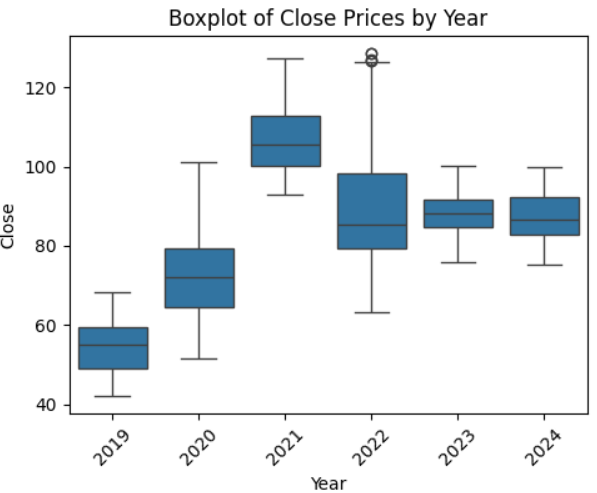
\includegraphics[width=1\textwidth]{Image/DatasetImg/SONY_Boxplot.png}
    \caption{SONY stock price's boxplot}
    \label{fig:1}
    \end{minipage}
    \hfill
    \begin{minipage}{0.23\textwidth}
    \centering
    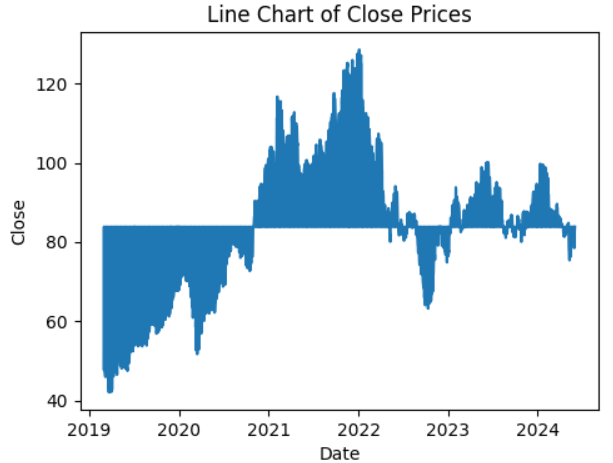
\includegraphics[width=1\textwidth]{Image/DatasetImg/SONY_LineChart.png}
    \caption{SONY stock price's histogram}
    \label{fig:2}
    \end{minipage}
\end{figure}

\begin{figure}[H]
    \centering
    \begin{minipage}{0.23\textwidth}
    \centering
    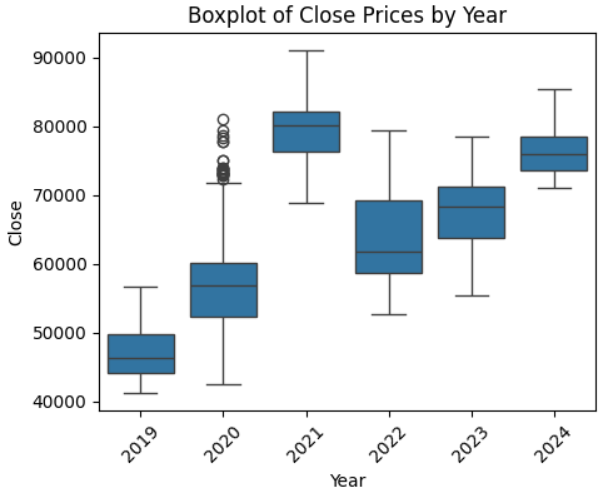
\includegraphics[width=1\textwidth]{Image/DatasetImg/SAMSUNG_Boxplot.png}
    \caption{SAMSUNG stock price's boxplot}
    \label{fig:1}
    \end{minipage}
    \hfill
    \begin{minipage}{0.23\textwidth}
    \centering
    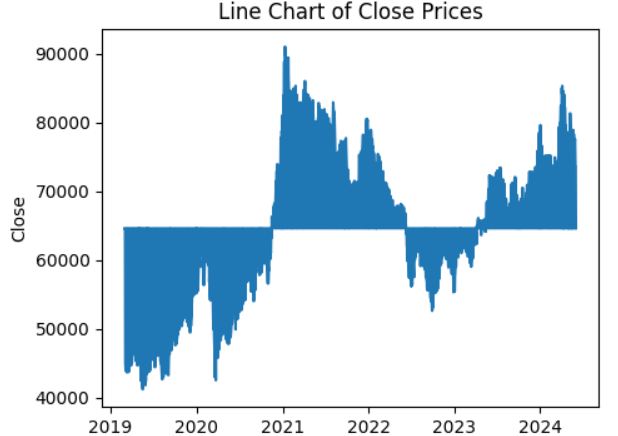
\includegraphics[width=1\textwidth]{Image/DatasetImg/SAMSUNG_LineChart.png}
    \caption{SAMSUNG stock price's histogram}
    \label{fig:2}
    \end{minipage}
\end{figure}

\begin{figure}[H]
    \centering
    \begin{minipage}{0.23\textwidth}
    \centering
    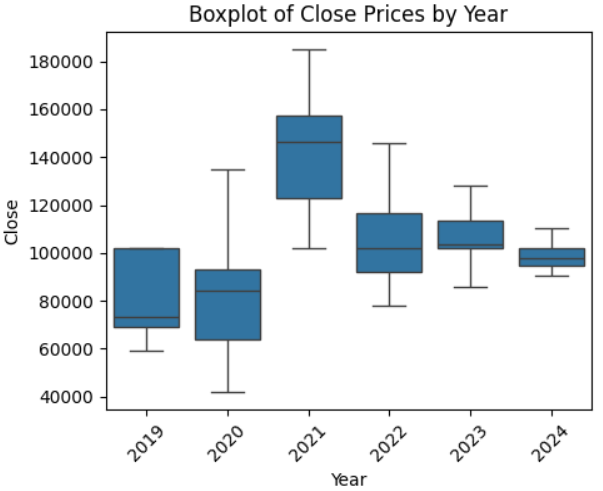
\includegraphics[width=1\textwidth]{Image/DatasetImg/LG_Boxplot.png}
    \caption{LG stock price's boxplot}
    \label{fig:1}
    \end{minipage}
    \hfill
    \begin{minipage}{0.23\textwidth}
    \centering
    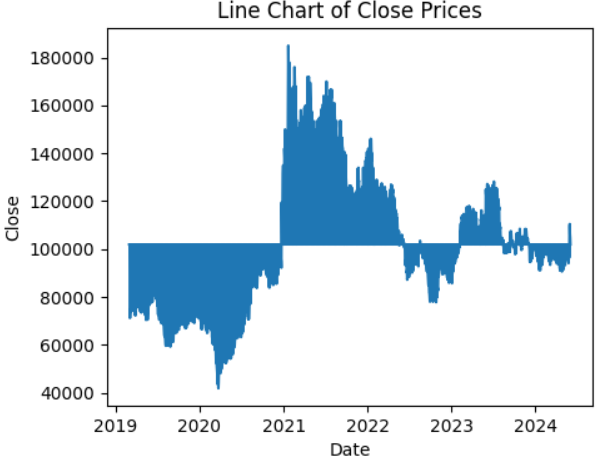
\includegraphics[width=1\textwidth]{Image/DatasetImg/LG_LineChart.png}
    \caption{LG stock price's histogram}
    \label{fig:2}
    \end{minipage}
\end{figure}


\subsection{TỶ LỆ PHÂN CHIA TẬP DỮ LIỆU}
 Tỷ lệ phân chia dữ liệu là một quyết định quan trọng trong việc xây dựng mô hình học máy. Trong bài nghiên cứu này, chúng tôi sẽ chia dữ liệu theo ba tỷ lệ khác nhau: 6:4, 7:3 và 8:2.
 Tỷ lệ 6:4, cho phép chúng ta có một tập kiểm thử tương đối lớn, giúp đánh giá mô hình một cách toàn diện hơn. Tuy nhiên, điều này cũng có nghĩa là chúng ta có ít dữ liệu hơn để huấn luyện mô hình, có thể ảnh hưởng đến khả năng học của mô hình.
 Tỷ lệ 7:3 cho phép chúng ta huấn luyện mô hình trên một lượng dữ liệu lớn hơn, trong khi vẫn đảm bảo có đủ dữ liệu để kiểm thử mô hình. Điều này giúp cải thiện hiệu suất của mô hình và khả năng tổng quát hóa.
 Tỷ lệ 8:2 cung cấp một sự cân nhắc giữa việc huấn luyện mô hình và đánh giá toàn diện trên tập dữ liệu kiểm thử, cung cấp một lựa chọn linh hoạt cho nhiều tình huống khác nhau.
 Nghiên cứu của chúng tôi nhấn mạnh tầm quan trọng của việc xem xét tỷ lệ phân chia dữ liệu để đảm bảo hiệu quả trong cả việc huấn luyện và đánh giá mô hình. Phương pháp tiếp cận tỉ mỉ này giúp đảm bảo rằng mô hình của chúng tôi có khả năng cung 
 cấp dự đoán chính xác và đáng tin cậy trong các tình huống thực tế. Đây không chỉ là một phần quan trọng của quá trình nghiên cứu của chúng tôi mà còn là một bước quan trọng để đảm bảo rằng kết quả của chúng tôi có thể được áp dụng và triển khai hiệu quả trong thực tế.

\subsection{CHỈ SỐ ĐÁNH GIÁ MÔ HÌNH}
\subsubsection{Mean Squared Error(MSE)}


Mean Squared Error (MSE) là một số liệu phổ biến được sử dụng trong các bài toán hồi quy. Về cơ bản, MSE tính sai số bình phương trung bình giữa các giá trị được dự đoán và giá trị thực tế. Đây là một thước đo chất lượng của mô hình dự đoán, luôn không âm và các giá trị càng gần 0 càng tốt.

Công thức tính MSE:
\[
\text{MSE} = \frac{1}{n} \sum_{i=1}^{n} (\hat{y}_i - y_i)^2
\]
trong đó:
\begin{itemize}
    \item $n$ là số điểm dữ liệu
    \item $y_i$ là giá trị quan sát
    \item $\hat{y}_i$ là giá trị dự đoán
\end{itemize}

Trong phân tích hồi quy, việc vẽ biểu đồ là một cách trực quan để xem xu hướng chung của dữ liệu. MSE cho bạn biết mức độ gần của đường hồi quy với tập hợp các điểm dữ liệu. Cụ thể, MSE đo khoảng cách từ các điểm dữ liệu đến đường hồi quy (các khoảng cách này là “sai số”) và bình phương chúng. Việc bình phương sai số là rất quan trọng vì nó loại bỏ các dấu âm và làm tăng trọng số của các sai số lớn.

Để giảm thiểu MSE, mô hình cần dự đoán chính xác hơn, tức là gần với dữ liệu thực tế hơn. Một ví dụ về hồi quy tuyến tính sử dụng phương pháp này là phương pháp bình phương nhỏ nhất. Phương pháp này đánh giá sự phù hợp của mô hình hồi quy tuyến tính với tập dữ liệu hai biến. Tuy nhiên, nó có giới hạn liên quan đến phân phối dữ liệu đã biết.

MSE càng thấp thì dự báo càng tốt.


\subsubsection{Root Mean Square Error(RMSE)}


Root Mean Square Error (RMSE) là căn bậc hai của mức trung bình các sai số bình phương. RMSE là độ lệch chuẩn của các phần dư (sai số dự đoán). Phần dư đo khoảng cách từ các điểm dữ liệu đến đường hồi quy, RMSE đo mức độ phân tán của các phần dư này, tức là mức độ tập trung của dữ liệu xung quanh đường hồi quy.

Công thức tính RMSE:
\[
\text{RMSE} = \sqrt{\frac{1}{n} \sum_{i=1}^{n} (\hat{y}_i - y_i)^2}
\]
trong đó:
\begin{itemize}
    \item $n$ là số điểm dữ liệu
    \item $y_i$ là giá trị thực tế
    \item $\hat{y}_i$ là giá trị dự đoán
\end{itemize}

Ảnh hưởng của mỗi lỗi đối với RMSE tỷ lệ với kích thước của lỗi bình phương, do đó các sai số lớn hơn có ảnh hưởng lớn đến RMSE một cách không cân xứng. Vì lý do này, RMSE nhạy cảm với các yếu tố ngoại lai. RMSE thường được sử dụng trong khí hậu học, dự báo, và phân tích hồi quy để xác minh kết quả thực nghiệm.

Khi các quan sát và dự báo được chuẩn hóa, RMSE có mối quan hệ trực tiếp với hệ số tương quan. Ví dụ, nếu hệ số tương quan là 1, RMSE sẽ bằng 0 vì tất cả các điểm nằm trên đường hồi quy (không có sai số).

RMSE luôn không âm, và giá trị 0 (hầu như không bao giờ đạt được trong thực tế) chỉ ra sự phù hợp hoàn hảo với dữ liệu. Nói chung, RMSE thấp hơn cho thấy mô hình tốt hơn so với RMSE cao hơn.

 

\subsubsection{Mean Absolute Percentage Error(MAPE)}

Mean Absolute Percentage Error (MAPE) là một số liệu được sử dụng để đo lường độ chính xác của các dự đoán trong các mô hình dự báo. MAPE tính toán sai số tuyệt đối trung bình dưới dạng phần trăm của giá trị thực tế, giúp đánh giá mức độ chính xác của dự đoán một cách dễ hiểu và so sánh dễ dàng giữa các tập dữ liệu khác nhau.

Công thức tính MAPE:
\[
\text{MAPE} = \frac{100\%}{n} \sum_{i=1}^{n} \left| \frac{y_i - \hat{y}_i}{y_i} \right|
\]
trong đó:
\begin{itemize}
    \item $n$ là số điểm dữ liệu
    \item $y_i$ là giá trị thực tế
    \item $\hat{y}_i$ là giá trị dự đoán
\end{itemize}

Ưu điểm của MAPE là nó biểu diễn sai số dưới dạng phần trăm, làm cho việc diễn giải và so sánh dễ dàng hơn. Tuy nhiên, MAPE có một số hạn chế, chẳng hạn như việc không xác định khi giá trị thực tế $y_i$ bằng 0 và có thể bị ảnh hưởng mạnh bởi các giá trị cực nhỏ của $y_i$, làm cho sai số phần trăm trở nên rất lớn.

MAPE thường được sử dụng trong các lĩnh vực như dự báo kinh tế, tài chính và quản lý chuỗi cung ứng để đánh giá độ chính xác của các mô hình dự báo.
\section{PHƯƠNG PHÁP}

\subsection{THUẬT TOÁN RNN}

 Mạng nơ-ron tái phát (RNN) là một loại mạng nơ-ron nhân tạo được thiết kế đặc biệt để xử lý các chuỗi dữ liệu có thứ tự, như chuỗi thời gian hoặc văn bản. Điểm đặc biệt của RNN là khả năng ghi nhớ và sử dụng thông tin từ các bước trước đó trong chuỗi, làm cho chúng rất hữu ích trong các bài toán như dịch máy, nhận dạng giọng nói và phân tích chuỗi thời gian.

\subsubsection{Cấu trúc và hoạt động của RNN}

RNN có cấu trúc đặc biệt với các kết nối hồi quy (recurrent connections), cho phép truyền thông tin ngược trở lại từ bước hiện tại về các bước trước đó. Điều này có nghĩa là tại mỗi bước thời gian \(t\), trạng thái ẩn \(a^{\langle t \rangle}\) được tính toán dựa trên trạng thái ẩn từ bước trước đó \(a^{\langle t-1 \rangle}\) và đầu vào hiện tại \(x^{\langle t \rangle}\).

\subsubsection{Công thức của RNN}

Công thức tính toán trong RNN có thể được biểu diễn như sau:

1. Trạng thái ẩn \(a^{\langle t \rangle}\):

\[
a^{\langle t \rangle} = g_1 \left( W_{aa} a^{\langle t-1 \rangle} + W_{ax} x^{\langle t \rangle} + b_a \right)
\]

2. Đầu ra \(y^{\langle t \rangle}\):

\[
y^{\langle t \rangle} = g_2 \left( W_{ya} a^{\langle t \rangle} + b_y \right)
\]

Trong đó:
\begin{itemize}
    \item \(W_{ax}\) và \(W_{aa}\) là ma trận trọng số cho đầu vào và trạng thái ẩn.
    \item \(W_{ya}\) là ma trận trọng số cho đầu ra.
    \item \(b_a\) và \(b_y\) là các bias tương ứng.
    \item \(g_1\) và \(g_2\) là các hàm kích hoạt, thường là hàm sigmoid hoặc hàm tanh cho trạng thái ẩn và hàm softmax cho đầu ra.
\end{itemize}

RNN rất mạnh mẽ nhưng cũng gặp khó khăn trong việc xử lý các chuỗi dài do vấn đề vanishing gradient. Để giải quyết vấn đề này, các biến thể của RNN như LSTM (Long Short-Term Memory) và GRU (Gated Recurrent Unit) đã được phát triển.

\begin{figure}
    \centering
    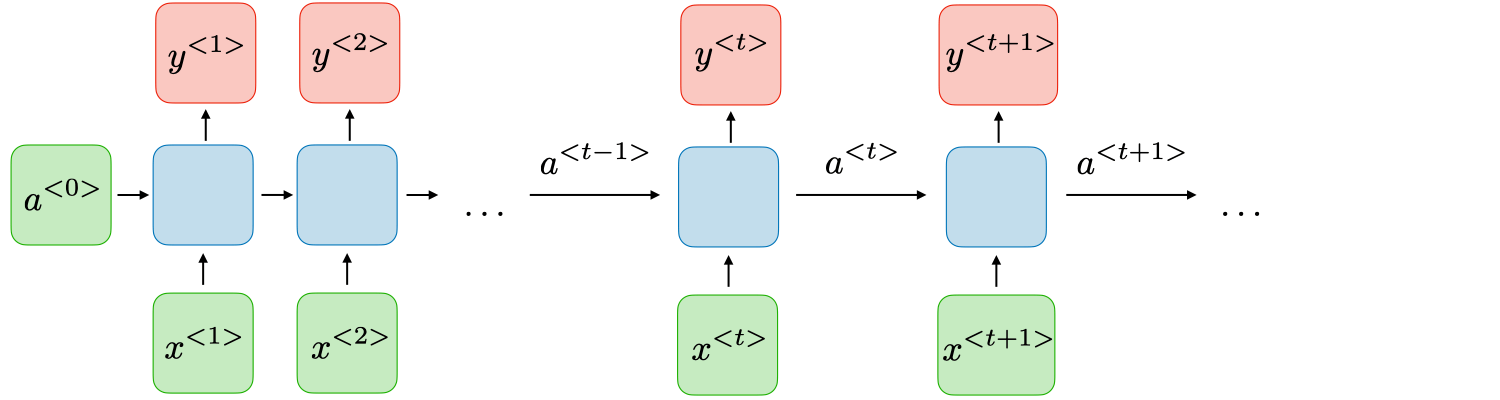
\includegraphics[width=0.5\linewidth]{image.png}
    \caption{Mô hình RNN đơn giản}
    \label{fig:rnn}
\end{figure}

RNN là một công cụ quan trọng trong học máy và trí tuệ nhân tạo, đặc biệt khi làm việc với dữ liệu tuần tự và có cấu trúc thời gian.


\subsection{THUẬT TOÁN LIGHTGBM}

LightGBM là một thuật toán học máy dựa trên cây quyết định, nó là một phần của họ các thuật toán tăng cường gradient.

Công thức cơ bản của LightGBM là:

\[
\hat{y}_i = \sum_{k=1}^{K} f_k(x_i), \quad f_k \in \mathcal{F}
\]

Trong đó:

\begin{align*}
&\hat{y}_i \text{ là giá trị dự đoán cho mẫu } i \\
&K \text{ là số lượng cây (trees) được sử dụng} \\
&f_k \text{ là cây thứ } k \text{ trong tập hợp các cây } \mathcal{F} \\
&x_i \text{ là vector đặc trưng cho mẫu } i
\end{align*}

LightGBM tối ưu hóa hàm mất mát bằng cách sử dụng thuật toán Gradient Boosting (tăng cường gradient).

Hàm mất mát thường được định nghĩa như sau:

\[
\text{loss}(\mathbf{y}, \hat{\mathbf{y}}) = \sum_{i=1}^{n} L(y_i, \hat{y}_i) + \sum_{k=1}^{K} \Omega(f_k)
\]

Trong đó:

\begin{align*}
&\mathbf{y} \text{ là vector các giá trị thực của các mẫu} \\
&\hat{\mathbf{y}} \text{ là vector các giá trị dự đoán} \\
&n \text{ là số lượng mẫu} \\
&L \text{ là hàm mất mát cho dự đoán và giá trị thực} \\
&\Omega \text{ là hàm điều chuẩn (regularization function) cho cây}
\end{align*}

LightGBM sử dụng các kỹ thuật như Gradient Boosting Decision Trees (GBDT) và histogram-based algorithm để tối ưu hóa hiệu suất tính toán và bộ nhớ.
\subsection{THUẬT TOÁN VARMA}
Mô hình VARMA thường được sử dụng để dự báo dữ liệu chuỗi thời gian đa biến . Mô hình VARMA là một mở rộng của mô hình ARMA trong chuỗi thời gian đơn biến (Lutkepohl, 2005; Wei, 1990) và được sử dụng với điều kiện dữ liệu phải là dừng theo thời gian (Lutkepohl, 2005). Mô hình VARMA (p,q) là sự kết hợp của mô hình VAR (p) và mô hình trung bình trượt vector (q) (VMA (q)).\\
 
    • Công thức:
    \begin{equation}
        \mathbf{y}_t = \mathbf{c} + \sum_{i=1}^{p} \mathbf{\Phi}_i \mathbf{y}_{t-i} + \sum_{j=1}^{q} \mathbf{\Theta}_j \boldsymbol{\epsilon}_{t-j} + \boldsymbol{\epsilon}_t
    \end{equation}  
Trong đó:  
    \begin{itemize}
      \item \( \mathbf{y}_t \) là vector của các biến tại thời điểm \( t \).
      \item \( \mathbf{c} \) là một vector hằng số.
      \item \( \mathbf{\Phi}_i \) là ma trận hệ số của chuỗi thời gian ( độ trễ, lag) \( i \) của mô hình AR.
      \item \( \mathbf{\Theta}_j \) là ma trận hệ số của chuỗi thời gian ( độ trễ, lag) \( j \) của mô hình MA.
      \item \( \boldsymbol{\epsilon}_t \) là vector của các nhiễu ngẫu nhiên tại thời điểm \( t \).
    \end{itemize} 
    \subsection{ARIMA}
    ARIMA model là viết tắt của cụm từ Autoregressive 
    Intergrated Moving Average. Mô hình sẽ biểu diễn phương trình hồi qui tuyến tính đa biến (multiple linear regression) của các biến đầu vào (còn gọi là biến phụ thuộc trong thống kê) là 2 thành phần chính:\\
    \begin{itemize}
        \item Auto regression: Kí hiệu là AR. Đây là thành phần tự hồi qui bao gồm tợp hợp các độ trễ của biến hiện tại. Độ trễ bậc p chính là giá trị lùi về quá khứ  bước thời gian của chuỗi. Độ trễ dài hoặc ngắn trong quá trình AR phụ thuộc vào tham số trễ.
    \end{itemize}
    \begin{itemize}
        \item Moving average: Quá trình trung bình trượt được hiểu là quá trình dịch chuyển hoặc thay đổi giá trị trung bình của chuổi theo thời gian. Do chuỗi của chúng ta được giả định là dừng nên quá trình thay đổi trung bình dường như là một chuỗi nhiễu trắng. Quá trình moving average sẽ tìm mối liên hệ về mặt tuyến tính giữa các phần tử ngẫu nhiên(stochastic term). 
    \end{itemize}
    \begin{itemize}
        \item Intergrated: Là quá trình đồng tích hợp hoặc lấy sai phân. Yêu cầu chung của các thuật toán trong time series là chuỗi phải đảm bảo tính dừng. Hầu hết các chuỗi đều tăng hoặc giảm theo thời gian. Do đó yếu tố tương quan giữa chúng chưa chắc là thực sự mà là do chúng cùng tương quan theo thời gian. Khi biến đổi sang chuỗi dừng, các nhân tố ảnh hưởng thời gian được loại bỏ và chuỗi sẽ dễ dự báo hơn. Để tạo thành chuỗi dừng, một phương pháp đơn giản nhất là chúng ta sẽ lấy sai phân. Một số chuỗi tài chính còn qui đổi sang logarit hoặc lợi suất. Bậc của sai phân để tạo thành chuỗi dừng còn gọi là bậc của quá trình đồng tích hợp (order of intergration).
    \end{itemize}
     • Công thức:
       \begin{equation}
           \mathbf{y}_t = \mathbf{c} + {\epsilon}_t + \sum_{i=1}^{p} \mathbf{\Phi}_i \mathbf{y}_{t-i} + \sum_{j=1}^{q} \mathbf{\Theta}_j \boldsymbol{\epsilon}_{t-j} 
       \end{equation}  
   Trong đó:  
       \begin{itemize}
         \item \( \mathbf{y}_t \) là giá trị của chuỗi thời gian tại thời điểm \( t \).
         \item \( \mathbf{c} \) là hằng số.
         \item \( \boldsymbol{\epsilon}_t \) là thành phần lỗi tại thời điểm thời điểm \( t \).
         \item \( \mathbf{\Phi}_i \) là hệ số của thành phần tự hồi quy (AR).
         \item \( \mathbf{\Theta}_j \) là hệ số của thành phần trung bình trượt (MA).
       \end{itemize} 

       \subsection{THUẬT TOÁN GRADIENT BOOSTING REGRESSION}
       Gradient Boosting Regressor là một thuật toán học máy mạnh mẽ được sử dụng cho các bài toán hồi quy. Nó kết hợp nhiều mô hình hồi quy đơn giản (thường là các cây quyết định) để tạo ra một mô hình dự đoán mạnh mẽ hơn. Thuật toán này dựa trên phương pháp boosting, một kỹ thuật học tập ensemble, trong đó các mô hình con được xây dựng liên tiếp nhau, với mỗi mô hình mới nhằm mục đích sửa lỗi của mô hình trước đó.\\
       Gradient Boosting là xây dựng mô hình dần dần bằng cách thêm vào các mô hình con mà mỗi mô hình mới tập trung vào việc sửa lỗi (residual) của các dự đoán trước đó. Điều này được thực hiện bằng cách tối ưu hóa gradient của hàm lỗi.\\
       Các bước thực hiện\\
       
       Khởi tạo mô hình ban đầu:\\
       Bắt đầu với một mô hình đơn giản, thường là giá trị trung bình của biến mục tiêu y.\\
       
       Tính toán residuals:\\
       Residuals là sai số giữa giá trị thực tế và giá trị dự đoán của mô hình hiện tại.\\
       
       Huấn luyện mô hình con:\\
       Huấn luyện một mô hình con (thường là một cây quyết định) để dự đoán residuals.\\
       
       Cập nhật mô hình hiện tại:\\
       Cập nhật mô hình hiện tại bằng cách thêm mô hình con mới với một trọng số (learning rate).\\
       
       Lặp lại:\\
       Lặp lại quá trình cho đến khi đạt được số lượng mô hình con mong muốn hoặc sai số giảm đến mức chấp nhận được.\\
       
       Ưu điểm và nhược điểm\\
       
       Ưu điểm:\\
       Hiệu quả cao trong việc giảm sai số và dự đoán chính xác.
       Linh hoạt với khả năng xử lý nhiều loại dữ liệu khác nhau.
       Có thể điều chỉnh nhiều tham số để tối ưu hóa hiệu suất.\\
       
       Nhược điểm:\\
       Tốn nhiều thời gian và tài nguyên tính toán.
       Dễ bị overfitting nếu không điều chỉnh cẩn thận các tham số.
       Khó khăn trong việc giải thích mô hình do tính phức tạp cao.\\

       \subsection{THUẬT TOÁN XGBoost}

       Thuật toán XGBoost là một thuật toán máy học thuộc loại ensemble learning, cụ thể là Gradient Boosting Framework. Nó sử dụng cây quyết định làm người học  cơ sở và sử dụng các kỹ thuật chính quy hóa để nâng cao khả năng khái quát của mô hình. XGBoost được sử dụng rộng rãi cho các tác vụ như hồi quy, phân loại và xếp hạng.
      
       XGBoost là một thuật toán máy học theo phương pháp học tập tổng hợp. Nó là xu hướng cho các nhiệm vụ học tập có giám sát, chẳng hạn như hồi quy và phân loại. XGBoost xây dựng mô hình dự đoán bằng cách kết hợp các dự đoán của nhiều mô hình riêng lẻ, thường là cây quyết định.
      
       XGBoost tối ưu hàm mục tiêu tại lần lặp t là:
      \begin{equation}
      \text{Obj}(t) = \sum_{i=1}^{n} l(y_i, \hat{y}_i^{(t-1)} + f_t(x_i)) + \Omega(f_t)
      \end{equation}
      
      Trong đó:
      \begin{itemize}
          \item \( l \) là hàm mất mát (loss function, ví dụ như MSE cho regression, logistic loss cho classification).
          \item \( y_i \) là giá trị thực tế của quan sát thứ \( i \).
          \item \( \hat{y}_i^{(t-1)} \) là dự đoán tại vòng lặp thứ \( t-1 \).
          \item \( f_t \) là cây quyết định được thêm vào tại vòng lặp thứ \( t \).
          \item \( \Omega(f_t) \) là hàm phạt (regularization term) giúp ngăn ngừa overfitting.
      \end{itemize}
      
       Các lợi ích và đặc điểm của mô hình XGBoost:\\
       - Độ chính xác cao: Bộ phân loại XGBoost nổi tiếng với độ chính xác cao và đã được chứng minh vượt trội hơn so với các thuật toán máy học khác trong nhiều nhiệm vụ dự đoán.\\
       - Khả năng mở rộng: XGBoost có khả năng mở rộng cao và có thể xử lý các bộ dữ liệu lớn với hàng triệu hàng và cột.\\
       - Hiệu quả: Nó được thiết kế để tính toán hiệu quả và có thể nhanh chóng huấn luyện các mô hình trên các bộ dữ liệu lớn.\\
       - Linh hoạt: XGBoost hỗ trợ nhiều loại dữ liệu và mục tiêu khác nhau, bao gồm hồi quy, phân loại và các vấn đề xếp hạng.\\
       - Chính quy hóa: Nó tích hợp các kỹ thuật chính quy để tránh hiện tượng quá khớp và cải thiện hiệu suất tổng quát.


    \subsection{THUẬT TOÁN N-BEAT}

    Thuật toán N-BEATS là một mô hình dự đoán chuỗi thời gian mạnh mẽ dựa trên một cấu trúc kiến trúc mạng nơ-ron đa tầng sâu. N-BEATS được thiết kế để có khả năng học được các biến đổi không tuyến tính và phức tạp trong dữ liệu chuỗi thời gian. Điểm nổi bật của N-BEATS là khả năng mở rộng và linh hoạt trong việc tùy chỉnh cấu trúc mạng. 

    Các đặc điểm chính: 
    
        + Cấu trúc mô hình : Mô hình N-BEATS thường bao gồm một hoặc nhiều khối có thể lặp lại. Mỗi khối bao gồm hai mạng nơ-ron: một mạng BackcastNet và một mạng ForecastNet. Cả hai mạng này thường có cấu trúc tương tự như Feedforward Neural Networks hoặc Convolutional Neural Networks.
    
        + Hàm mất mát : N-BEATS thường sử dụng hàm mất mát như Mean Absolute Error (MAE) hoặc Mean Squared Error (MSE) giữa dự đoán và giá trị thực tế của chuỗi thời gian. 
    
        + Quá trình huấn luyện : Mô hình N-BEATS được huấn luyện thông qua việc tối ưu hóa hàm mất mát bằng các phương pháp tối ưu hóa như gradient descent hoặc các biến thể của nó, như Adam hoặc RMSprop.
    
        + Backcast và Forecast:
        
            Backcast : Quá trình dự đoán các giá trị trong quá khứ của chuỗi thời gian. Trong quá trình này, mô hình sẽ sử dụng các giá trị quan sát được trong quá khứ để dự đoán giá trị tại một thời điểm cụ thể trong quá khứ. Quá trình này giúp mô hình học được cách biến đổi và ảnh hưởng của dữ liệu đầu vào đối với các giá trị trong quá khứ, từ đó cung cấp thông tin cần thiết để dự đoán tương lai.
    
            Porecast: Quá trình dự đoán các giá trị trong tương lai của chuỗi thời gian. Trong quá trình này, mô hình sẽ sử dụng các giá trị quan sát được trong hiện tại và quá khứ để dự đoán giá trị tại một thời điểm cụ thể trong tương lai. Quá trình này cho phép mô hình học được cách dữ liệu hiện tại và quá khứ ảnh hưởng đến các giá trị trong tương lai, từ đó cung cấp dự đoán cho các giá trị trong tương lai của chuỗi thời gian

\section{THỰC NGHIỆM}

\subsection{MÔ HÌNH DỰ ĐOÁN }
\subsubsection{ARIMA}
\begin{figure}[H]
    \centering
    \begin{minipage}{0.15\textwidth}
    \centering
    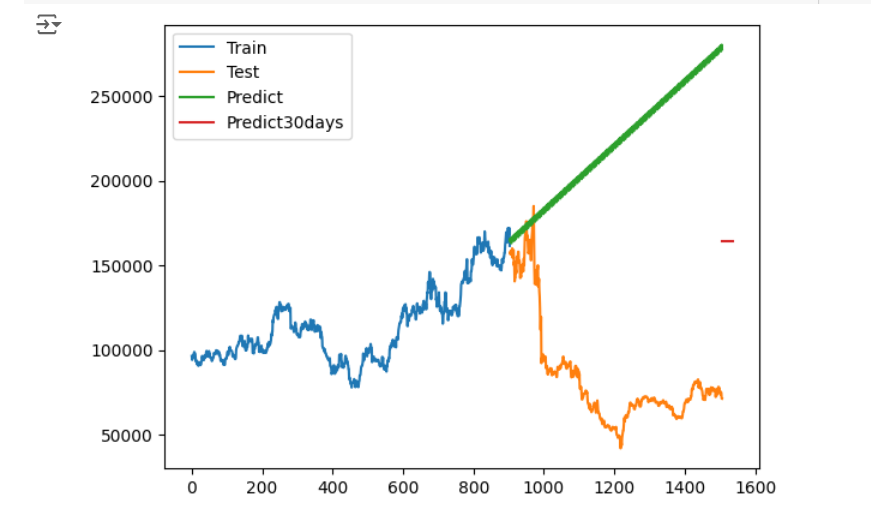
\includegraphics[width=1\textwidth]{Image/ARIMA/30_6_4_LG_Arima.png}
   
    \label{fig:1}
    \end{minipage}%
    \begin{minipage}{0.15\textwidth}
    \centering
    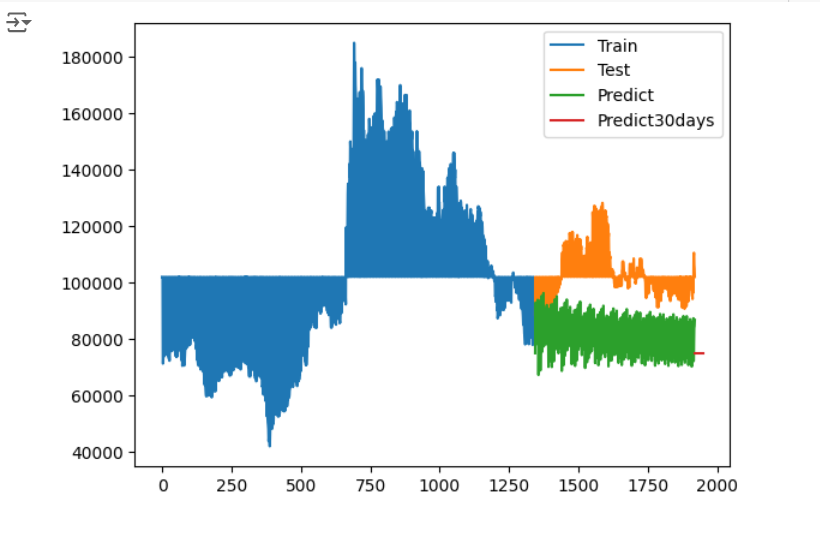
\includegraphics[width=1\textwidth]{Image/ARIMA/30_7_3_LG_Arima.png}
  
    \label{fig:2}
    \end{minipage}%
    \begin{minipage}{0.15\textwidth}
    \centering
    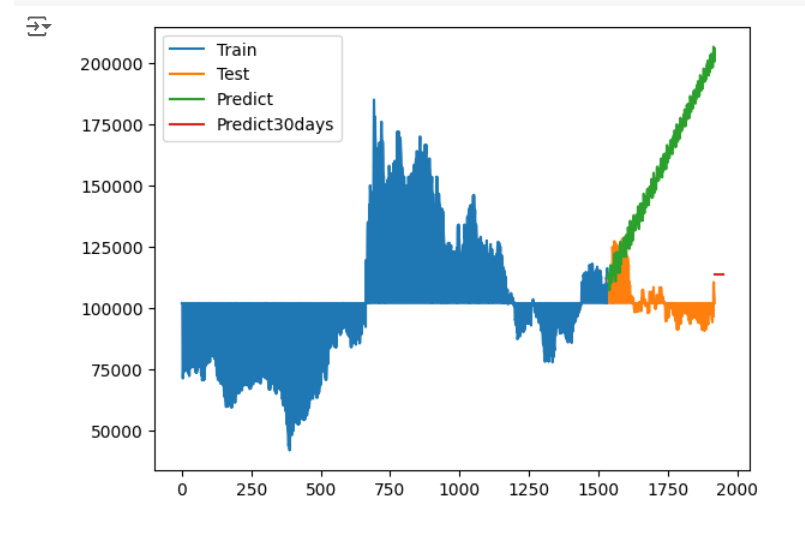
\includegraphics[width=1\textwidth]{Image/ARIMA/30_8_2_LG_Arima.png}

    \label{fig:3}
    \end{minipage}
    \caption{LG 30 DAYS  6:4, 7:3, 8:2 }
\end{figure}

\begin{figure}[H]
    \centering
    \begin{minipage}{0.15\textwidth}
    \centering
    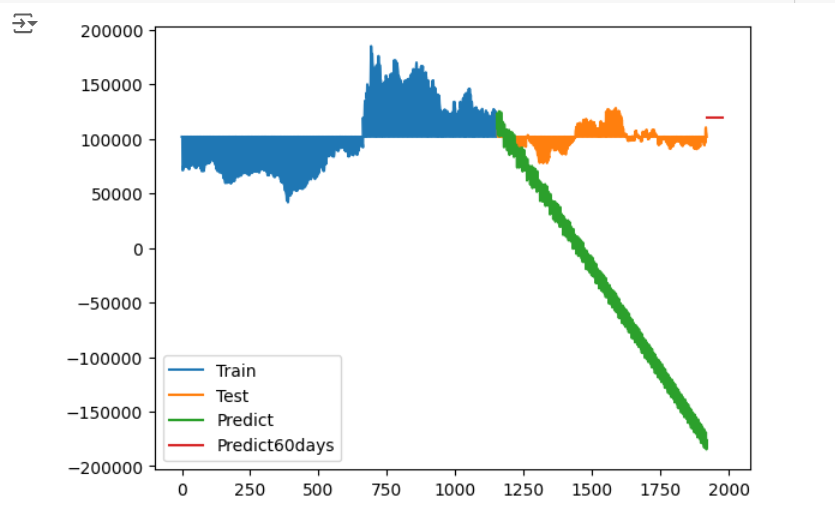
\includegraphics[width=1\textwidth]{Image/ARIMA/60_6_4_LG_Arima.png}
   
    \label{fig:1}
    \end{minipage}%
    \begin{minipage}{0.15\textwidth}
    \centering
    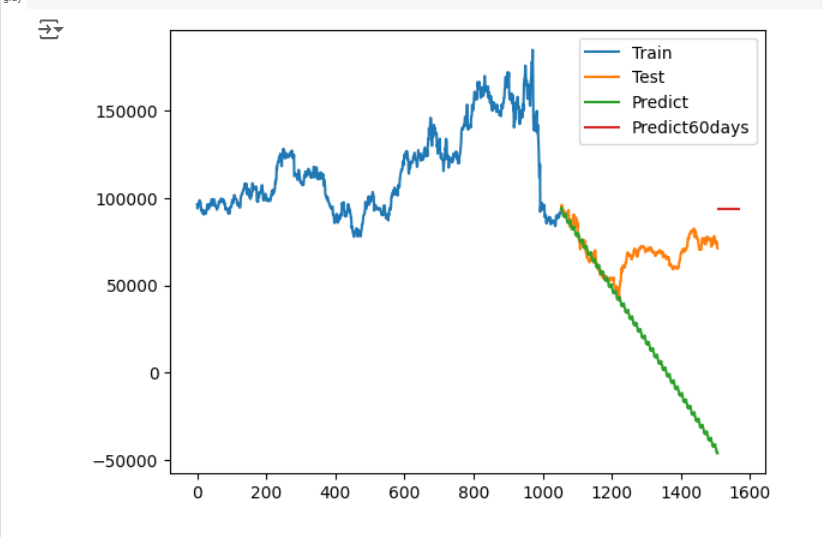
\includegraphics[width=1\textwidth]{Image/ARIMA/60_7_3_LG_Arima.png}
  
    \label{fig:2}
    \end{minipage}%
    \begin{minipage}{0.15\textwidth}
    \centering
    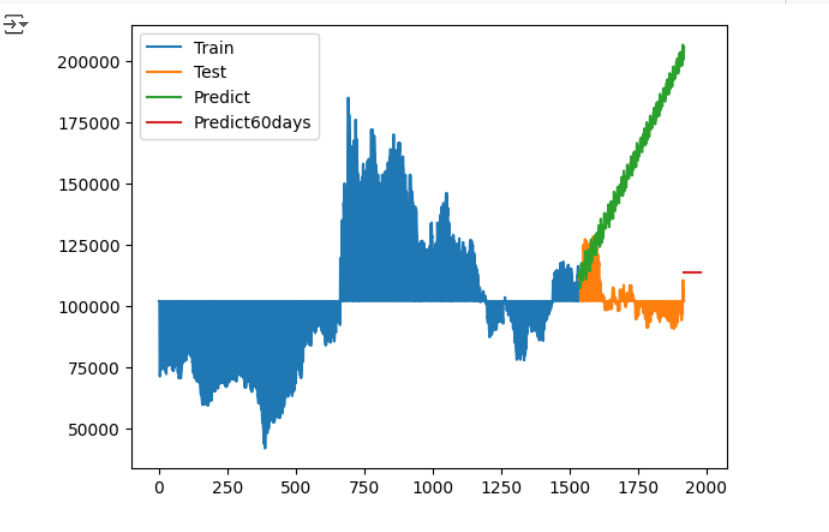
\includegraphics[width=1\textwidth]{Image/ARIMA/60_8_2_LG_Arima.png}

    \label{fig:3}
    \end{minipage}
    \caption{LG 60 DAYS  6:4, 7:3, 8:2 }
\end{figure}

\begin{figure}[H]
    \centering
    \begin{minipage}{0.15\textwidth}
    \centering
    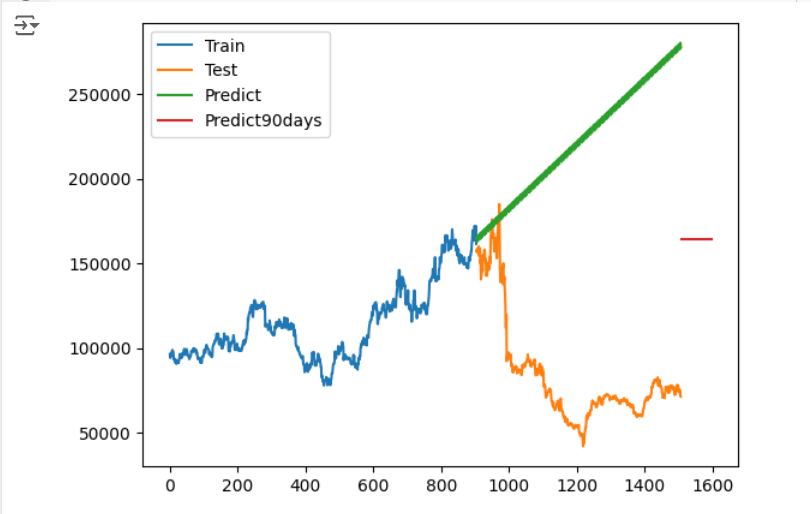
\includegraphics[width=1\textwidth]{Image/ARIMA/90_6_4_LG_Arima.png}
   
    \label{fig:1}
    \end{minipage}%
    \begin{minipage}{0.15\textwidth}
    \centering
    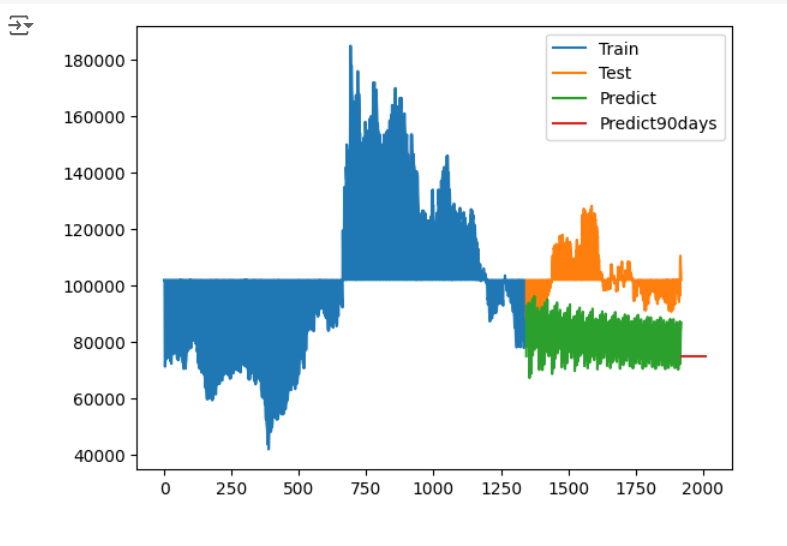
\includegraphics[width=1\textwidth]{Image/ARIMA/90_7_3_LG_Arima.png}
  
    \label{fig:2}
    \end{minipage}%
    \begin{minipage}{0.15\textwidth}
    \centering
    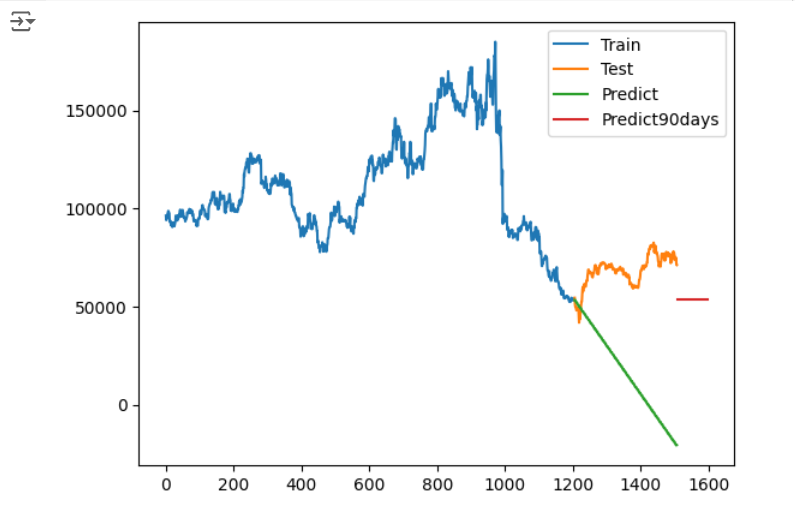
\includegraphics[width=1\textwidth]{Image/ARIMA/90_8_2_LG_Arima.png}

    \label{fig:3}
    \end{minipage}
    \caption{LG 90 DAYS  6:4, 7:3, 8:2 }
\end{figure}

\begin{figure}[H]
    \centering
    \begin{minipage}{0.15\textwidth}
    \centering
    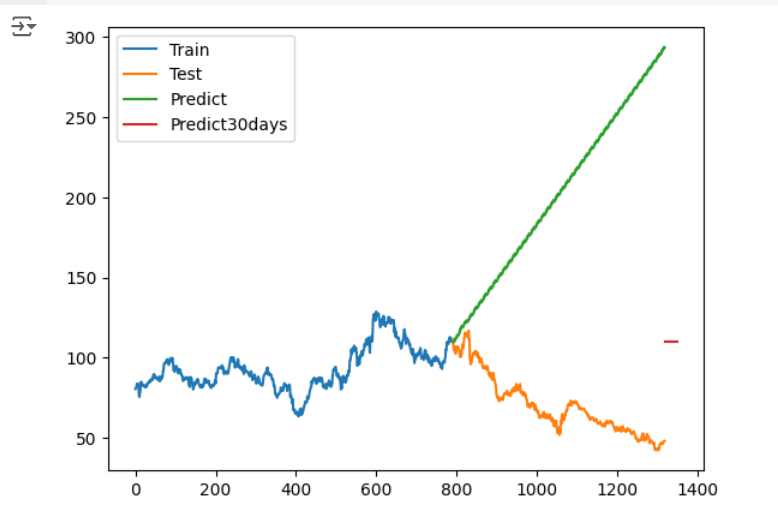
\includegraphics[width=1\textwidth]{Image/ARIMA/30_6_4_SONY_Arima.png}
   
    \label{fig:1}
    \end{minipage}%
    \begin{minipage}{0.15\textwidth}
    \centering
    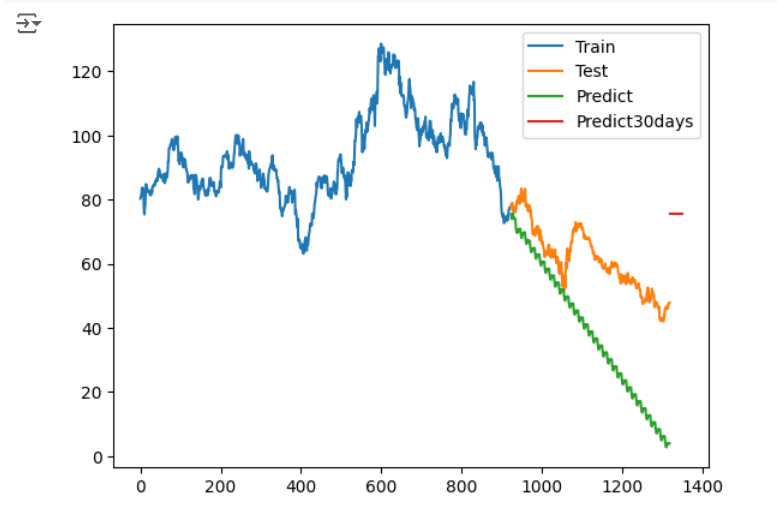
\includegraphics[width=1\textwidth]{Image/ARIMA/30_7_3_SONY_Arima.png}
  
    \label{fig:2}
    \end{minipage}%
    \begin{minipage}{0.15\textwidth}
    \centering
    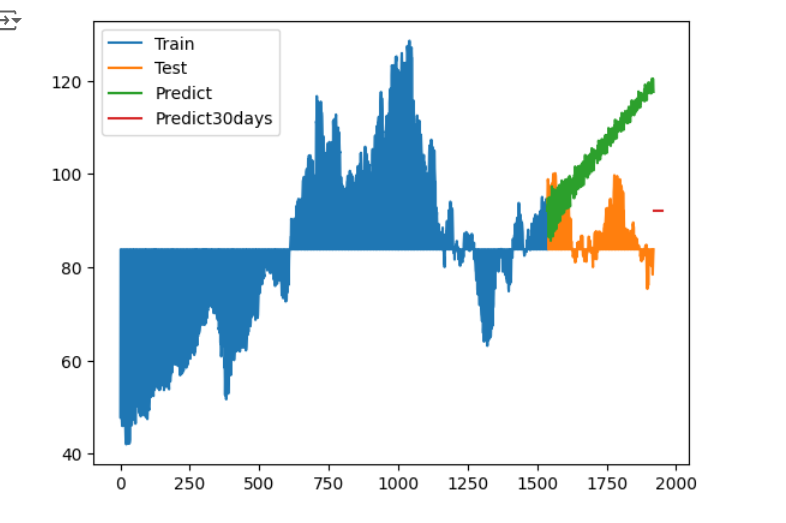
\includegraphics[width=1\textwidth]{Image/ARIMA/30_8_2_SONY_Arima.png}

    \label{fig:3}
    \end{minipage}
    \caption{SONY 30 DAYS  6:4, 7:3, 8:2 }
\end{figure}

\begin{figure}[H]
    \centering
    \begin{minipage}{0.15\textwidth}
    \centering
    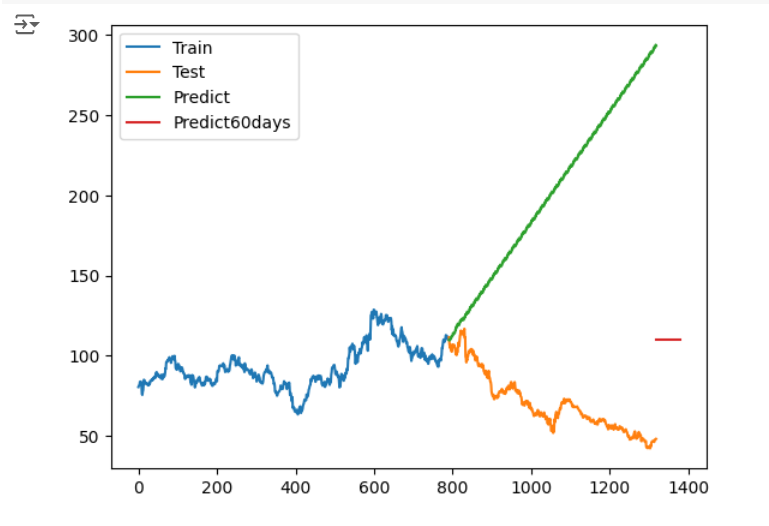
\includegraphics[width=1\textwidth]{Image/ARIMA/60_6_4_SONY_Arima.png}
   
    \label{fig:1}
    \end{minipage}%
    \begin{minipage}{0.15\textwidth}
    \centering
    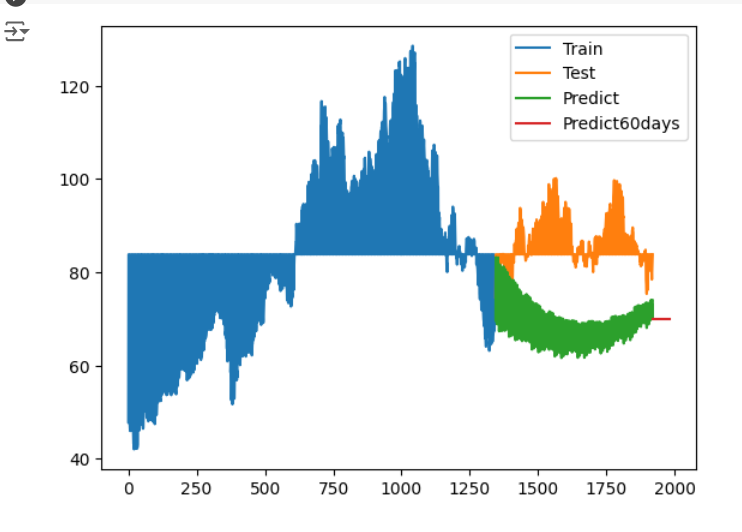
\includegraphics[width=1\textwidth]{Image/ARIMA/60_7_3_SONY_Arima.png}
  
    \label{fig:2}
    \end{minipage}%
    \begin{minipage}{0.15\textwidth}
    \centering
    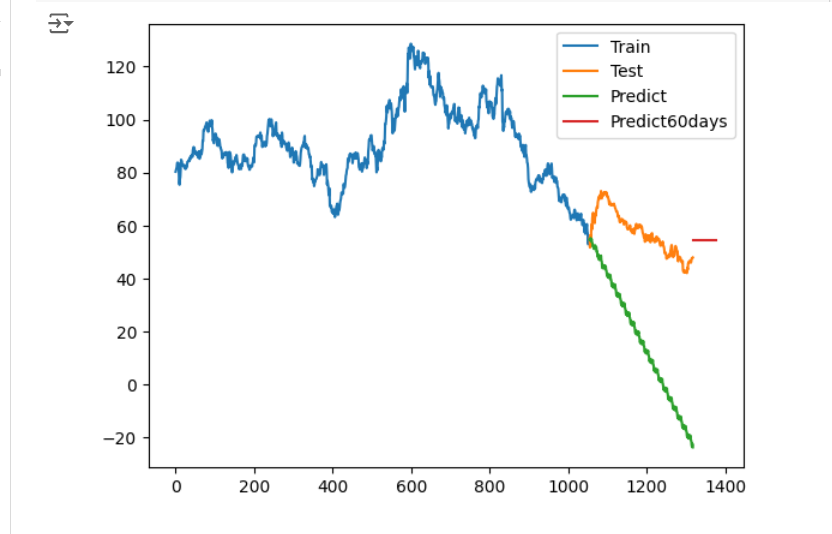
\includegraphics[width=1\textwidth]{Image/ARIMA/60_8_2_SONY_Arima.png}

    \label{fig:3}
    \end{minipage}
    \caption{SONY 60 DAYS  6:4, 7:3, 8:2 }
\end{figure}


\begin{figure}[H]
    \centering
    \begin{minipage}{0.15\textwidth}
    \centering
    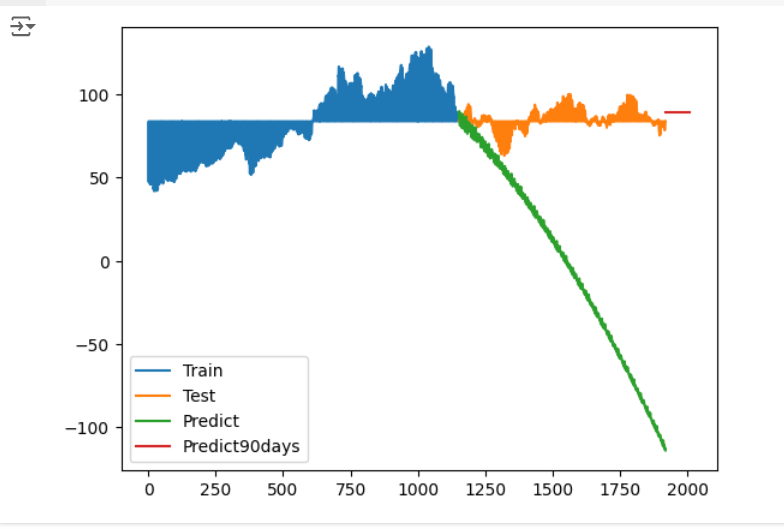
\includegraphics[width=1\textwidth]{Image/ARIMA/90_6_4_SONY_Arima.png}
   
    \label{fig:1}
    \end{minipage}%
    \begin{minipage}{0.15\textwidth}
    \centering
    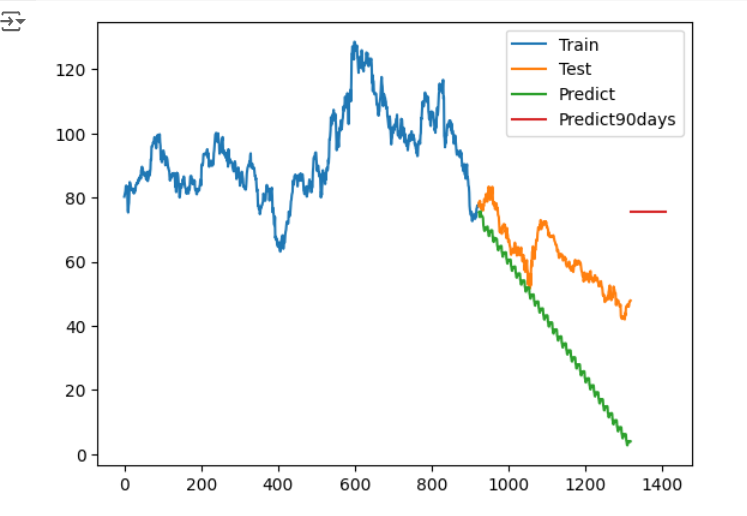
\includegraphics[width=1\textwidth]{Image/ARIMA/90_7_3_SONY_Arima.png}
  
    \label{fig:2}
    \end{minipage}%
    \begin{minipage}{0.15\textwidth}
    \centering
    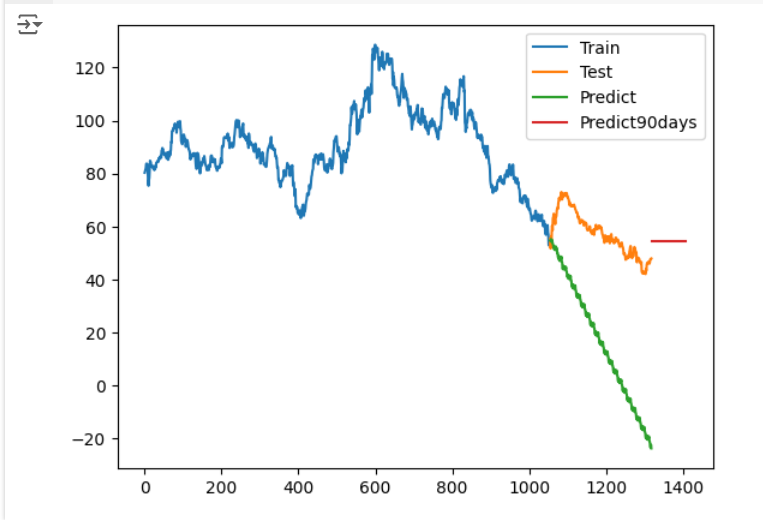
\includegraphics[width=1\textwidth]{Image/ARIMA/90_8_2_SONY_Arima.png}

    \label{fig:3}
    \end{minipage}
    \caption{SONY 90 DAYS  6:4, 7:3, 8:2 }
\end{figure}


\begin{figure}[H]
    \centering
    \begin{minipage}{0.15\textwidth}
    \centering
    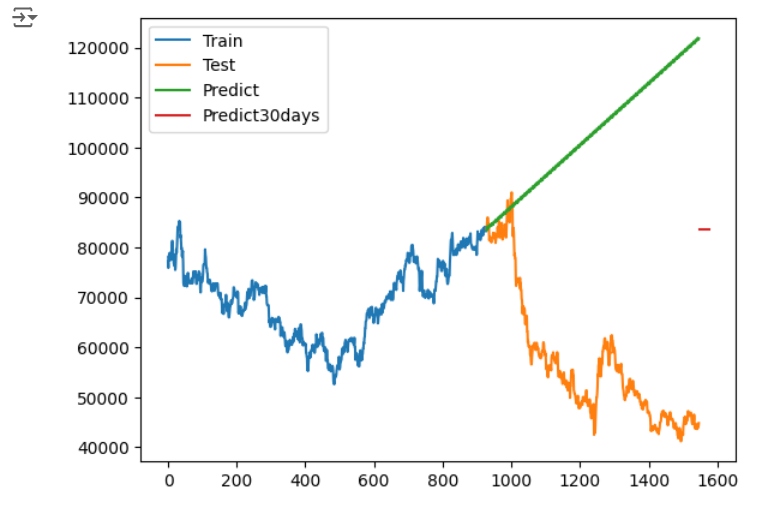
\includegraphics[width=1\textwidth]{Image/ARIMA/30_6_4_SAMSUNG_Arima.png}
   
    \label{fig:1}
    \end{minipage}%
    \begin{minipage}{0.15\textwidth}
    \centering
    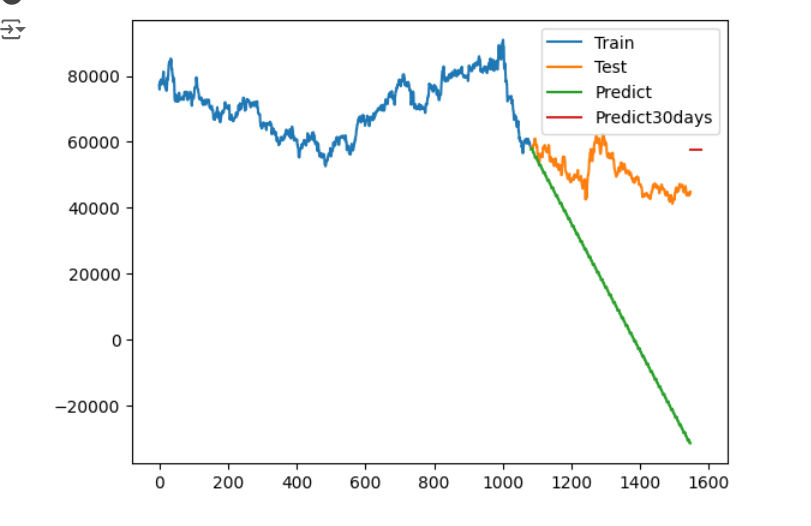
\includegraphics[width=1\textwidth]{Image/ARIMA/30_7_3_SAMSUNG_Arima.png}
  
    \label{fig:2}
    \end{minipage}%
    \begin{minipage}{0.15\textwidth}
    \centering
    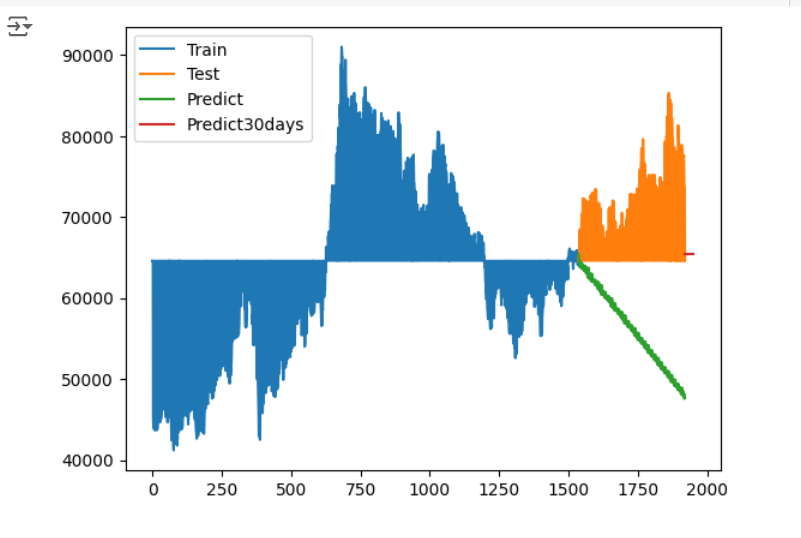
\includegraphics[width=1\textwidth]{Image/ARIMA/30_8_2_SAMSUNG_Arima.png}

    \label{fig:3}
    \end{minipage}
    \caption{SAMSUNG 30 DAYS  6:4, 7:3, 8:2 }
\end{figure}

\begin{figure}[H]
    \centering
    \begin{minipage}{0.15\textwidth}
    \centering
    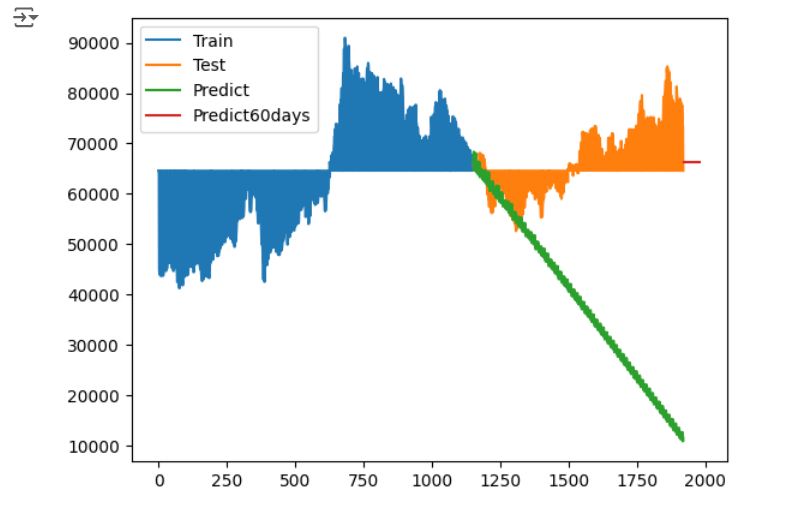
\includegraphics[width=1\textwidth]{Image/ARIMA/60_6_4_SAMSUNG_Arima.png}
   
    \label{fig:1}
    \end{minipage}%
    \begin{minipage}{0.15\textwidth}
    \centering
    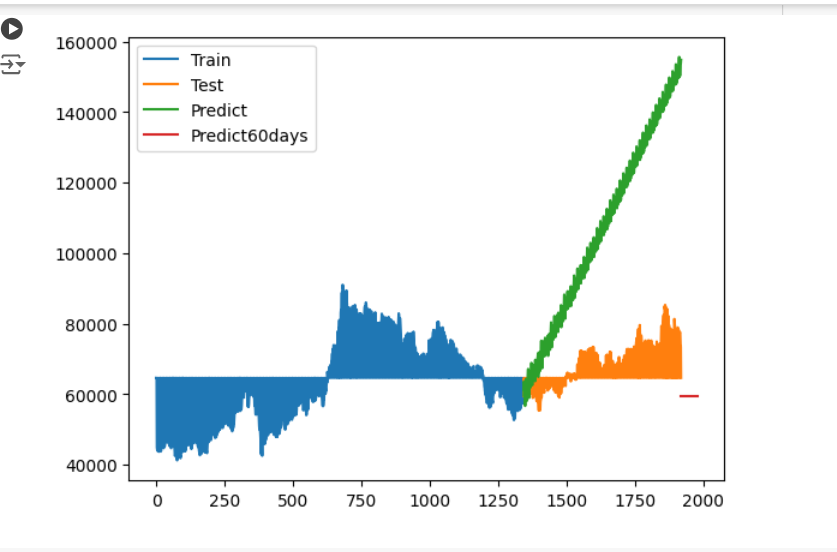
\includegraphics[width=1\textwidth]{Image/ARIMA/60_7_3_SAMSUNG_Arima.png}
  
    \label{fig:2}
    \end{minipage}%
    \begin{minipage}{0.15\textwidth}
    \centering
    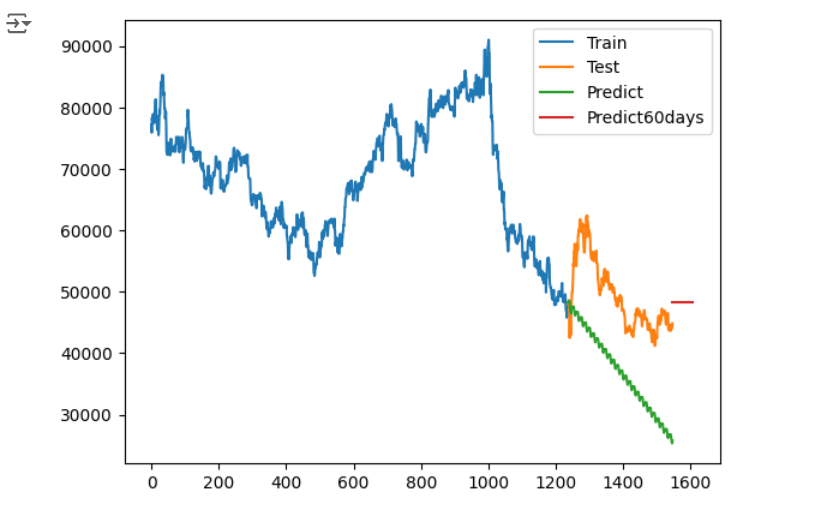
\includegraphics[width=1\textwidth]{Image/ARIMA/60_8_2_SAMSUNG_Arima.png}

    \label{fig:3}
    \end{minipage}
    \caption{SAMSUNG 60 DAYS  6:4, 7:3, 8:2 }
\end{figure}

\begin{figure}[H]
    \centering
    \begin{minipage}{0.15\textwidth}
    \centering
    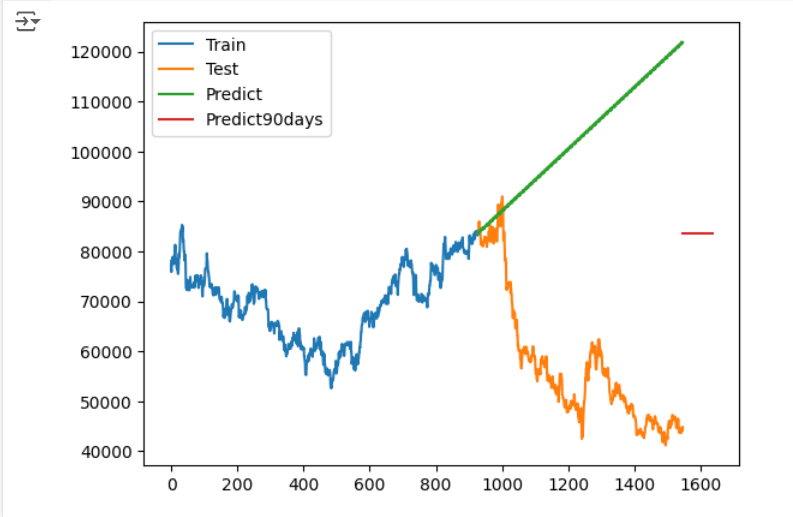
\includegraphics[width=1\textwidth]{Image/ARIMA/90_6_4_SAMSUNG_Arima.png}
   
    \label{fig:1}
    \end{minipage}%
    \begin{minipage}{0.15\textwidth}
    \centering
    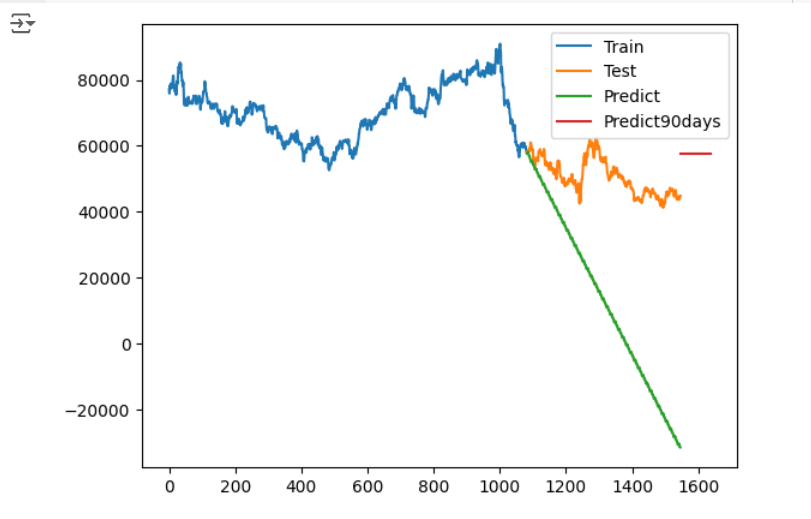
\includegraphics[width=1\textwidth]{Image/ARIMA/90_7_3_SAMSUNG_Arima.png}
  
    \label{fig:2}
    \end{minipage}%
    \begin{minipage}{0.15\textwidth}
    \centering
    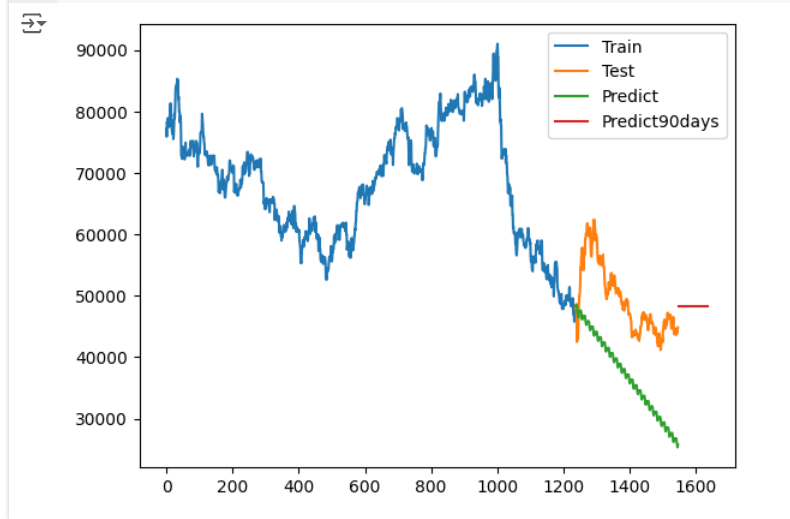
\includegraphics[width=1\textwidth]{Image/ARIMA/90_8_2_SAMSUNG_Arima.png}

    \label{fig:3}
    \end{minipage}
    \caption{SAMSUNG 90 DAYS  6:4, 7:3, 8:2 }
\end{figure} 
\subsubsection{LINEAR REGRESSION}



\begin{figure}[H]
    \centering
    \begin{minipage}{0.15\textwidth}
    \centering
    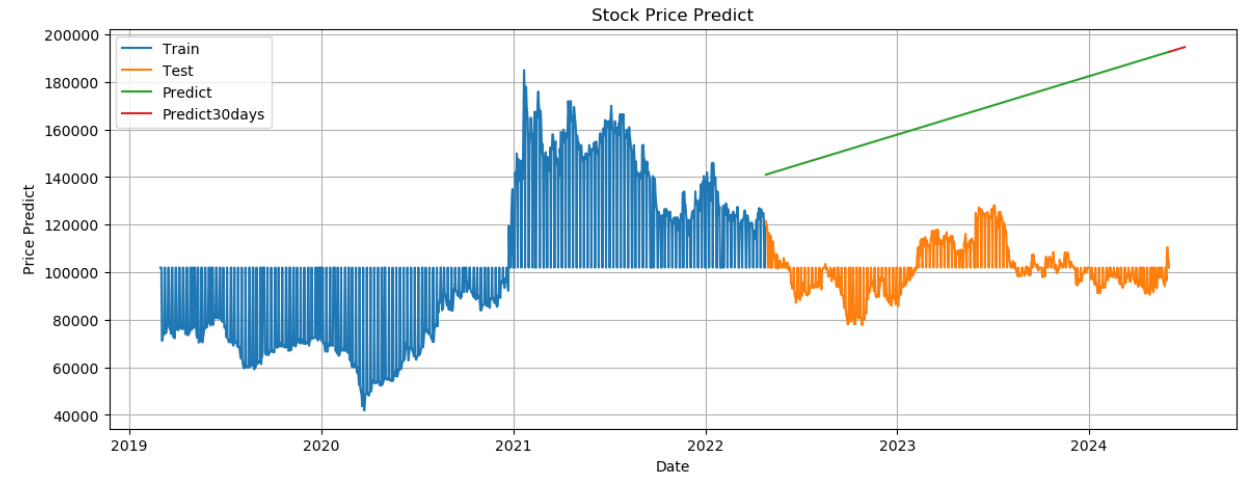
\includegraphics[width=1\textwidth]{Image/Linear/Linear_LG_6_4_30DAYS.png}
   
    \label{fig:1}
    \end{minipage}%
    \begin{minipage}{0.15\textwidth}
    \centering
    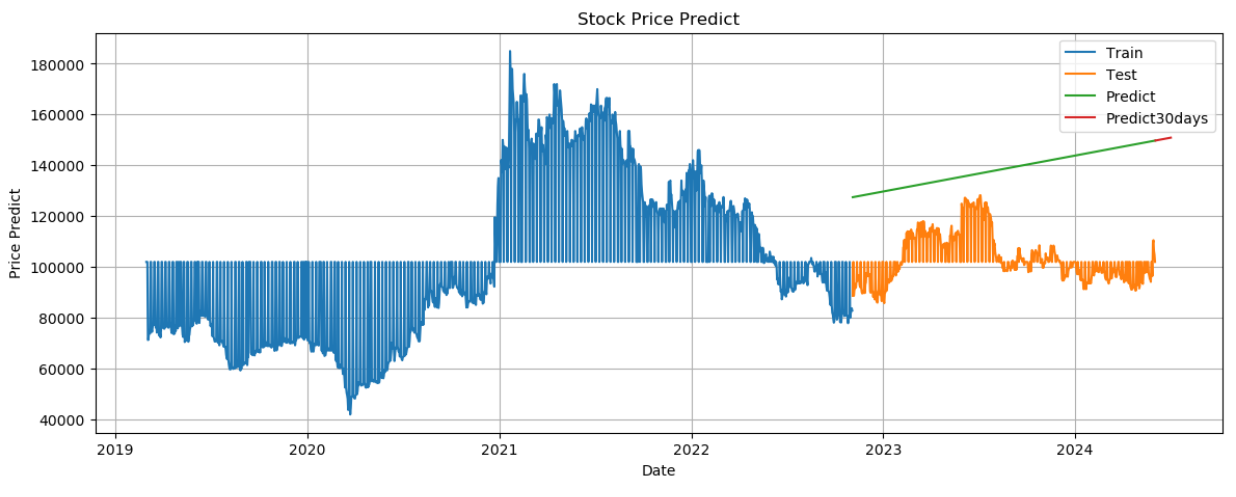
\includegraphics[width=1\textwidth]{Image/Linear/Linear_LG_7_3_30DAYS.png}
  
    \label{fig:2}
    \end{minipage}%
    \begin{minipage}{0.15\textwidth}
    \centering
    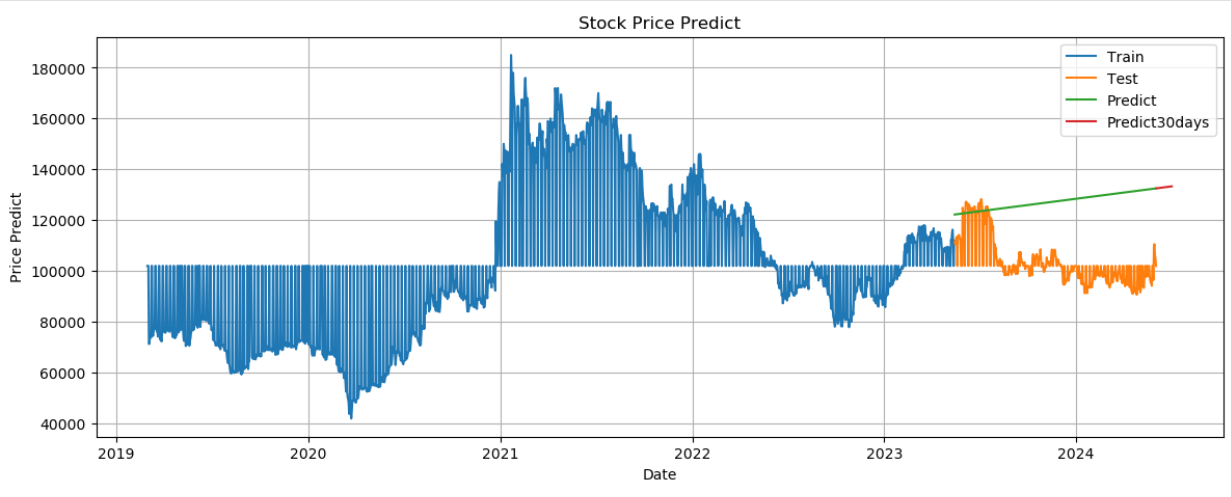
\includegraphics[width=1\textwidth]{Image/Linear/Linear_LG_8_2_30DAYS.png}

    \label{fig:3}
    \end{minipage}
    \caption{LG 30 DAYS  6:4, 7:3, 8:2 }
\end{figure}

\begin{figure}[H]
    \centering
    \begin{minipage}{0.15\textwidth}
    \centering
    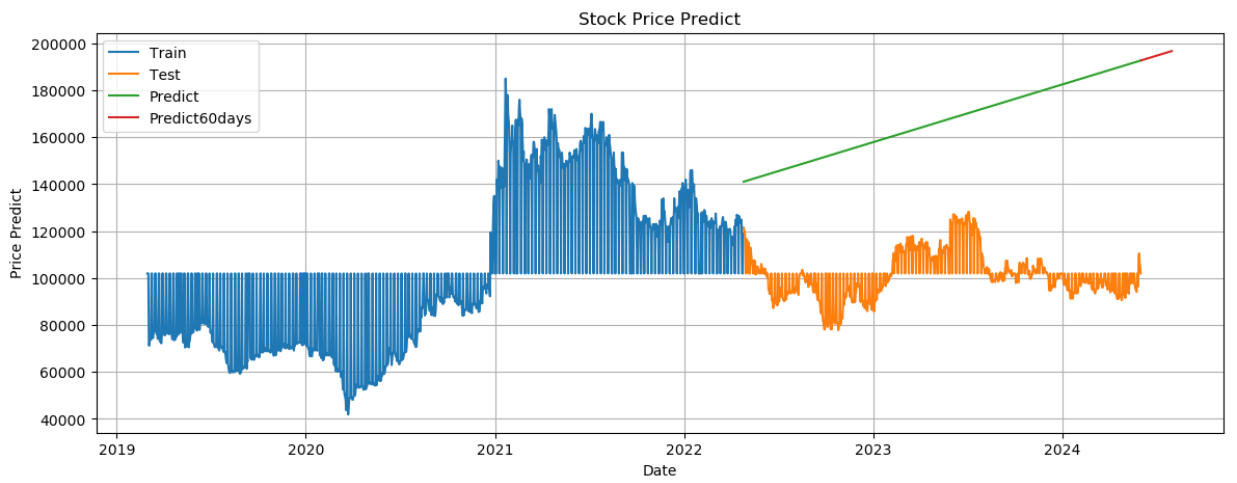
\includegraphics[width=1\textwidth]{Image/Linear/Linear_LG_6_4_60DAYS.png}
   
    \label{fig:1}
    \end{minipage}%
    \begin{minipage}{0.15\textwidth}
    \centering
    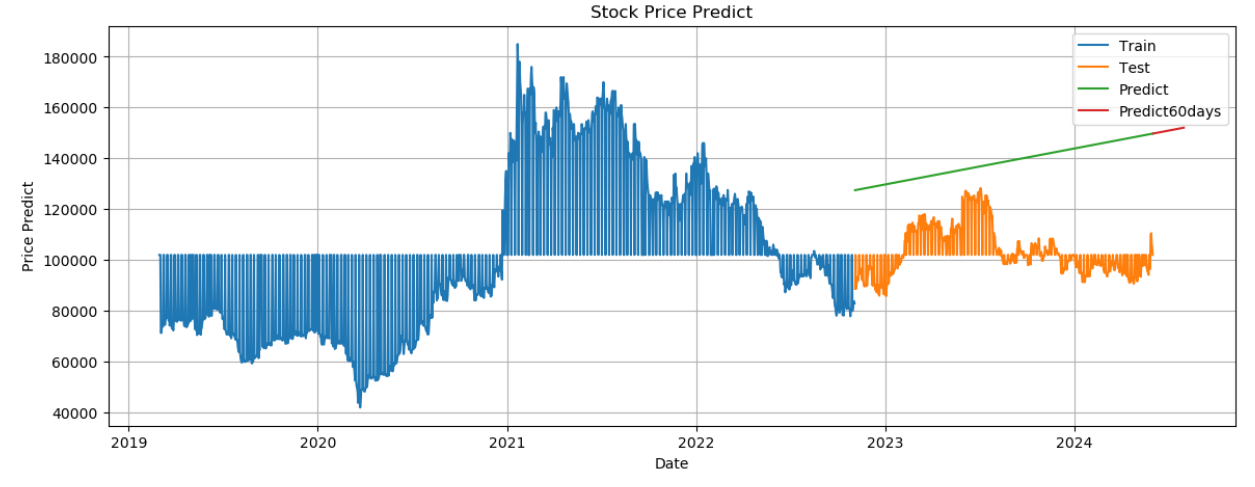
\includegraphics[width=1\textwidth]{Image/Linear/Linear_LG_7_3_60DAYS.png}
  
    \label{fig:2}
    \end{minipage}%
    \begin{minipage}{0.15\textwidth}
    \centering
    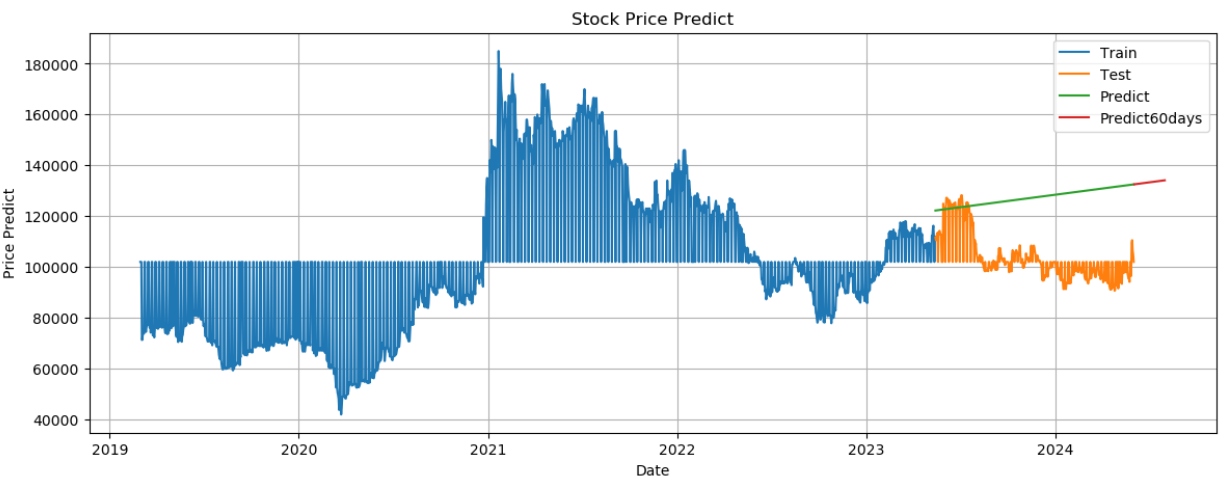
\includegraphics[width=1\textwidth]{Image/Linear/Linear_LG_8_2_60DAYS.png}

    \label{fig:3}
    \end{minipage}
    \caption{LG 60 DAYS  6:4, 7:3, 8:2 }
\end{figure}

\begin{figure}[H]
    \centering
    \begin{minipage}{0.15\textwidth}
    \centering
    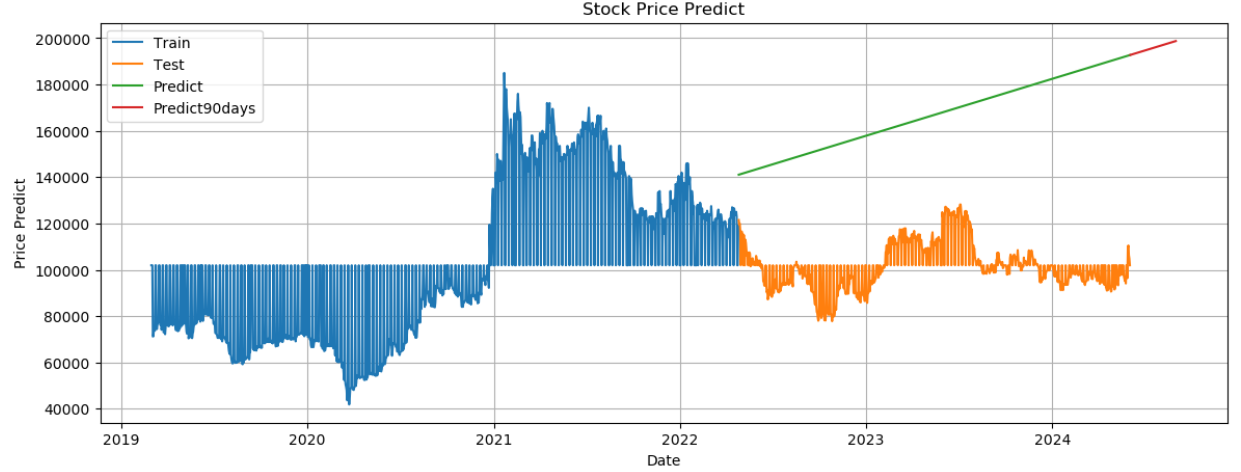
\includegraphics[width=1\textwidth]{Image/Linear/Linear_LG_6_4_90DAYS.png}
   
    \label{fig:1}
    \end{minipage}%
    \begin{minipage}{0.15\textwidth}
    \centering
    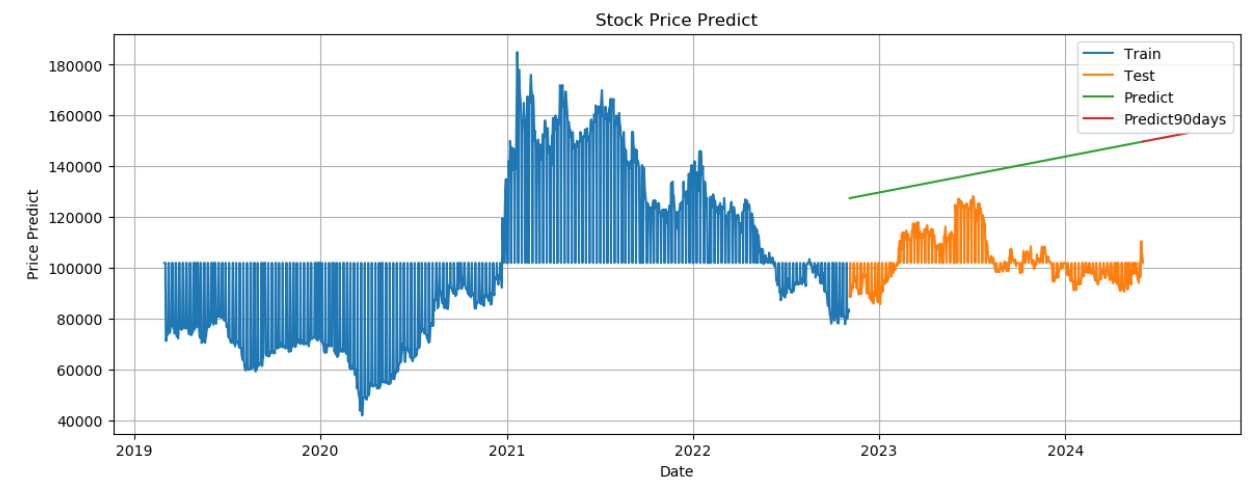
\includegraphics[width=1\textwidth]{Image/Linear/Linear_LG_7_3_90DAYS.png}
  
    \label{fig:2}
    \end{minipage}%
    \begin{minipage}{0.15\textwidth}
    \centering
    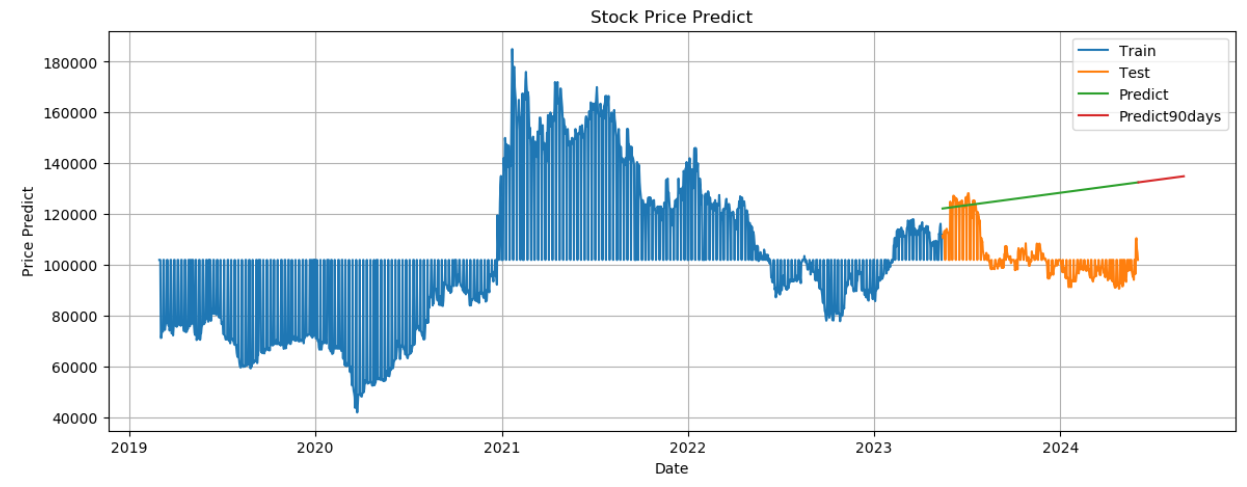
\includegraphics[width=1\textwidth]{Image/Linear/Linear_LG_8_2_90DAYS.png}

    \label{fig:3}
    \end{minipage}
    \caption{LG 90 DAYS  6:4, 7:3, 8:2 }
\end{figure}

\begin{figure}[H]
    \centering
    \begin{minipage}{0.15\textwidth}
    \centering
    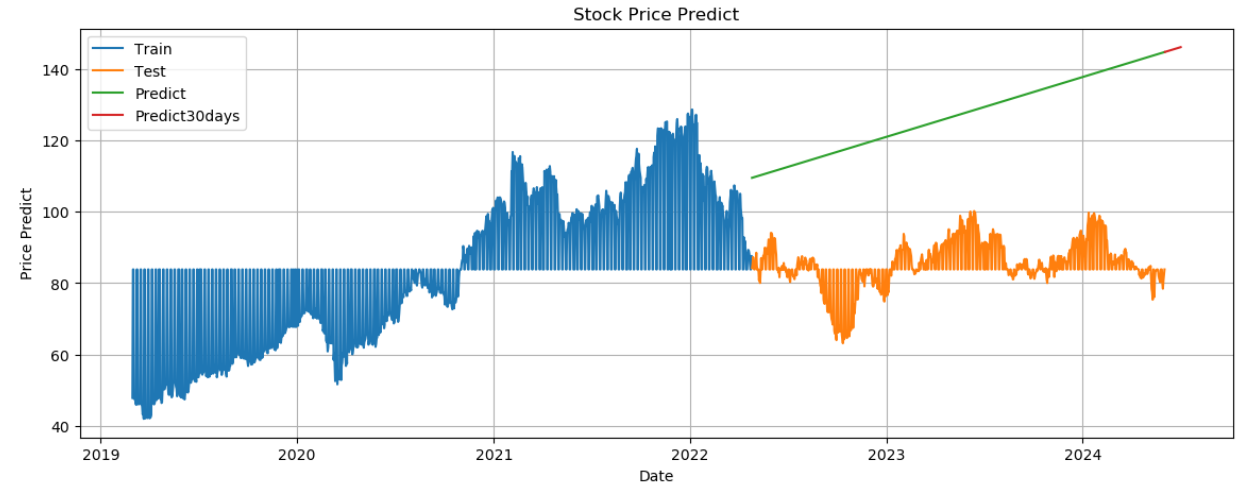
\includegraphics[width=1\textwidth]{Image/Linear/Linear_SONY_6_4_30DAYS.png}
   
    \label{fig:1}
    \end{minipage}%
    \begin{minipage}{0.15\textwidth}
    \centering
    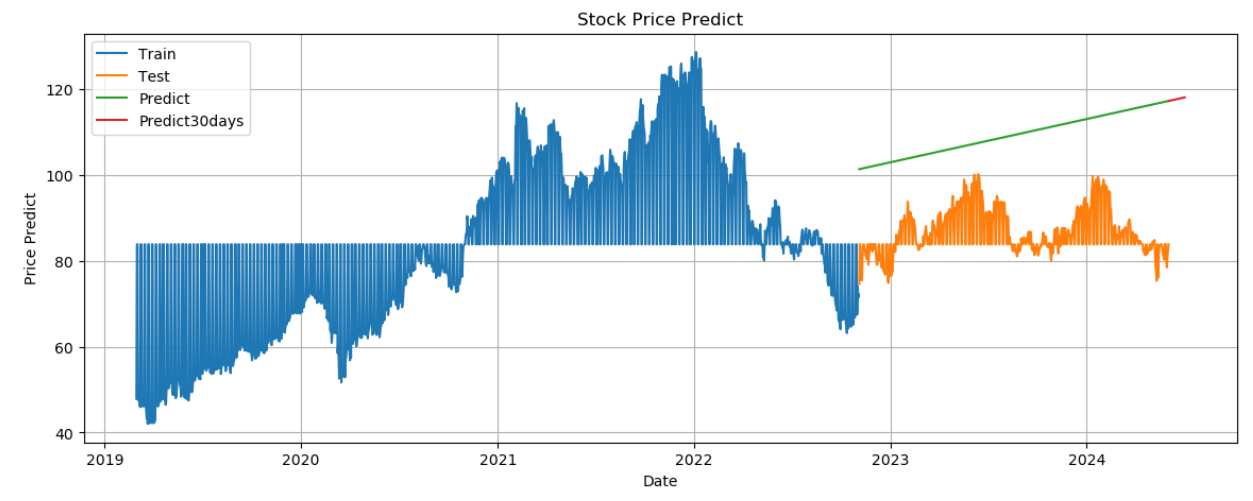
\includegraphics[width=1\textwidth]{Image/Linear/Linear_SONY_7_3_30DAYS.png}
  
    \label{fig:2}
    \end{minipage}%
    \begin{minipage}{0.15\textwidth}
    \centering
    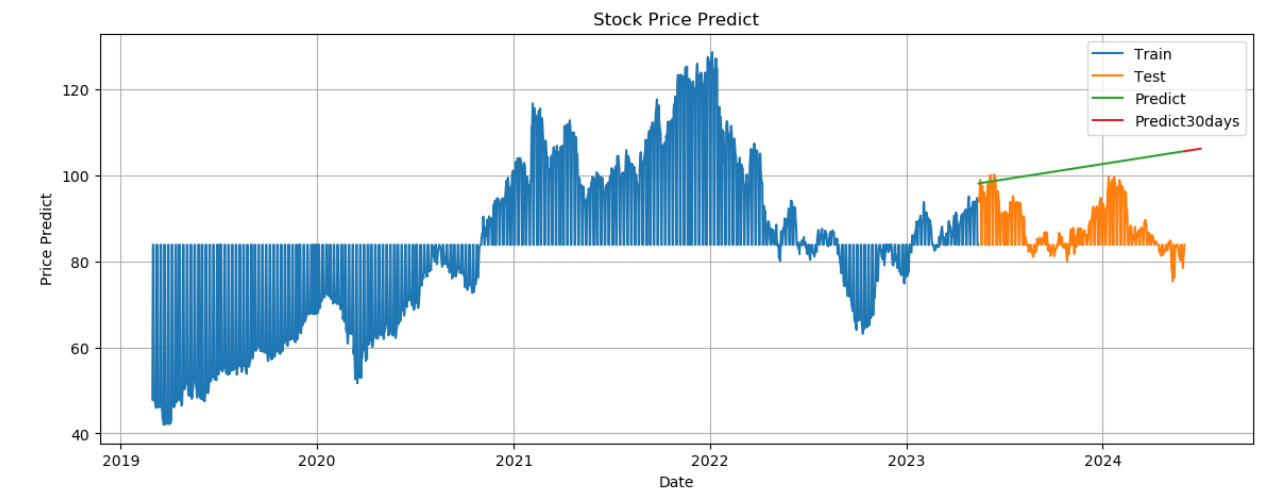
\includegraphics[width=1\textwidth]{Image/Linear/Linear_SONY_8_2_30DAYS.png}

    \label{fig:3}
    \end{minipage}
    \caption{SONY 30 DAYS  6:4, 7:3, 8:2 }
\end{figure}

\begin{figure}[H]
    \centering
    \begin{minipage}{0.15\textwidth}
    \centering
    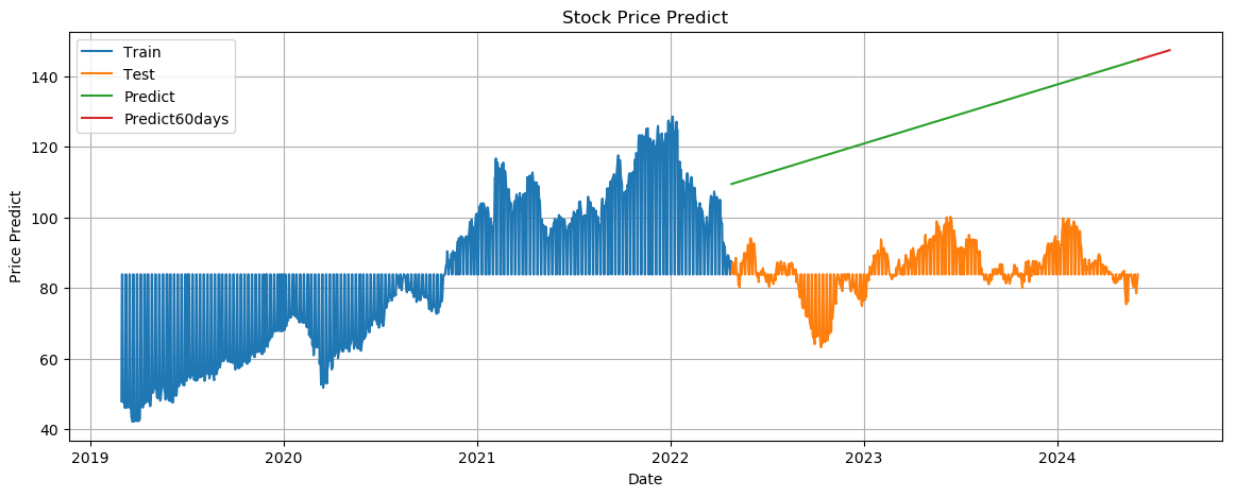
\includegraphics[width=1\textwidth]{Image/Linear/Linear_SONY_6_4_60DAYS.png}
   
    \label{fig:1}
    \end{minipage}%
    \begin{minipage}{0.15\textwidth}
    \centering
    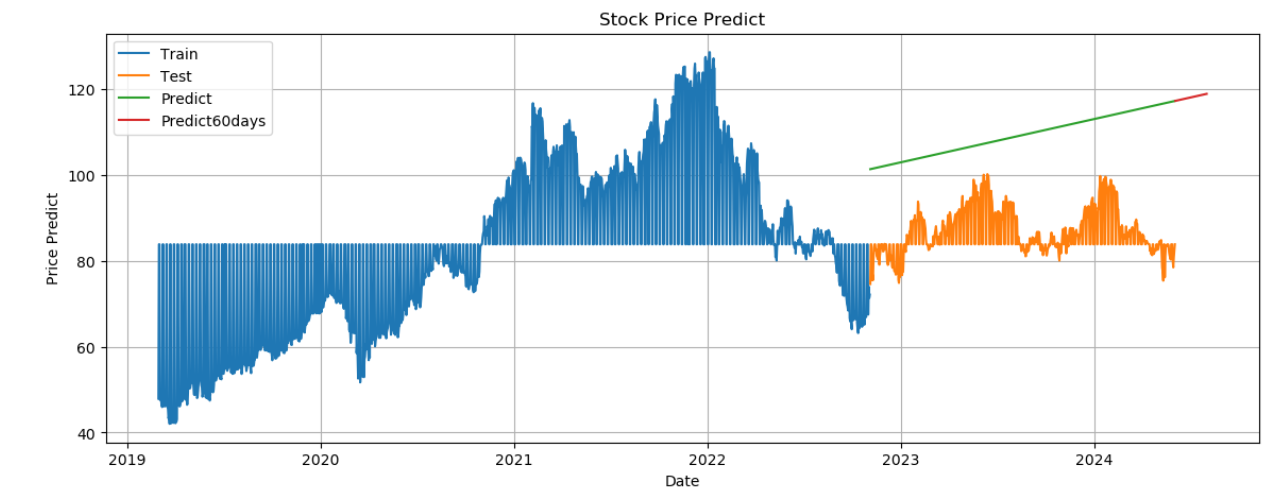
\includegraphics[width=1\textwidth]{Image/Linear/Linear_SONY_7_3_60DAYS.png}
  
    \label{fig:2}
    \end{minipage}%
    \begin{minipage}{0.15\textwidth}
    \centering
    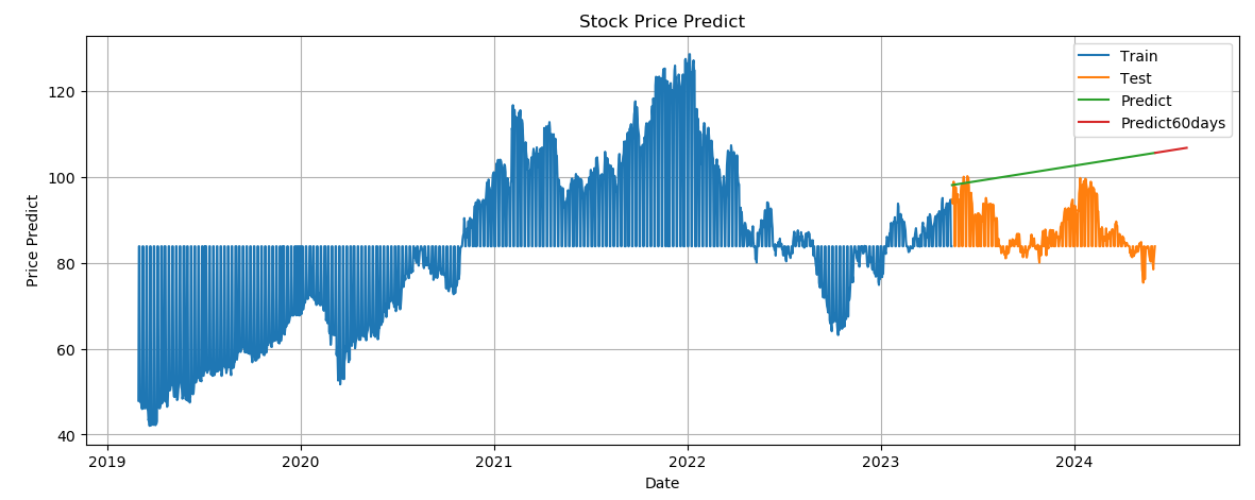
\includegraphics[width=1\textwidth]{Image/Linear/Linear_SONY_8_2_60DAYS.png}

    \label{fig:3}
    \end{minipage}
    \caption{SONY 60 DAYS  6:4, 7:3, 8:2 }
\end{figure}


\begin{figure}[H]
    \centering
    \begin{minipage}{0.15\textwidth}
    \centering
    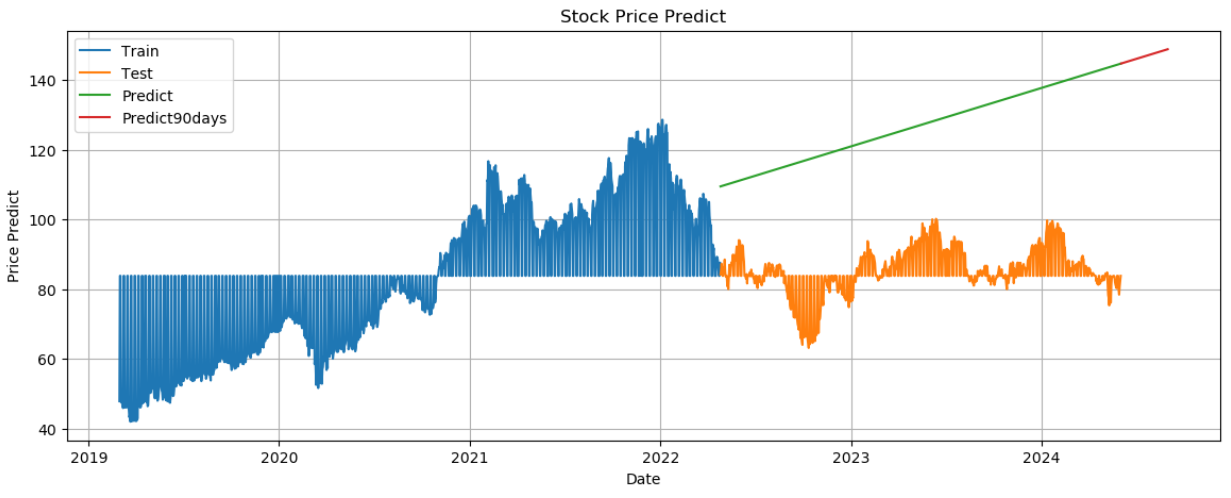
\includegraphics[width=1\textwidth]{Image/Linear/Linear_SONY_6_4_90DAYS.png}
   
    \label{fig:1}
    \end{minipage}%
    \begin{minipage}{0.15\textwidth}
    \centering
    \includegraphics[width=1\textwidth]{Image/Linear/Linear_SONY_7_3_90DAYS.png}
  
    \label{fig:2}
    \end{minipage}%
    \begin{minipage}{0.15\textwidth}
    \centering
    \includegraphics[width=1\textwidth]{Image/Linear/Linear_SONY_8_2_90DAYS.png}

    \label{fig:3}
    \end{minipage}
    \caption{SONY 90 DAYS  6:4, 7:3, 8:2 }
\end{figure}


\begin{figure}[H]
    \centering
    \begin{minipage}{0.15\textwidth}
    \centering
    \includegraphics[width=1\textwidth]{Image/Linear/Linear_SAMSUNG_6_4_30DAYS.png}
   
    \label{fig:1}
    \end{minipage}%
    \begin{minipage}{0.15\textwidth}
    \centering
    \includegraphics[width=1\textwidth]{Image/Linear/Linear_SAMSUNG_7_3_30DAYS.png}
  
    \label{fig:2}
    \end{minipage}%
    \begin{minipage}{0.15\textwidth}
    \centering
    \includegraphics[width=1\textwidth]{Image/Linear/Linear_SAMSUNG_8_2_30DAYS.png}

    \label{fig:3}
    \end{minipage}
    \caption{SAMSUNG 30 DAYS  6:4, 7:3, 8:2 }
\end{figure}

\begin{figure}[H]
    \centering
    \begin{minipage}{0.15\textwidth}
    \centering
    \includegraphics[width=1\textwidth]{Image/Linear/Linear_SAMSUNG_6_4_60DAYS.png}
   
    \label{fig:1}
    \end{minipage}%
    \begin{minipage}{0.15\textwidth}
    \centering
    \includegraphics[width=1\textwidth]{Image/Linear/Linear_SAMSUNG_7_3_60DAYS.png}
  
    \label{fig:2}
    \end{minipage}%
    \begin{minipage}{0.15\textwidth}
    \centering
    \includegraphics[width=1\textwidth]{Image/Linear/Linear_SAMSUNG_8_2_60DAYS.png}

    \label{fig:3}
    \end{minipage}
    \caption{SAMSUNG 60 DAYS  6:4, 7:3, 8:2 }
\end{figure}

\begin{figure}[H]
    \centering
    \begin{minipage}{0.15\textwidth}
    \centering
    \includegraphics[width=1\textwidth]{Image/Linear/Linear_SAMSUNG_6_4_90DAYS.png}
   
    \label{fig:1}
    \end{minipage}%
    \begin{minipage}{0.15\textwidth}
    \centering
    \includegraphics[width=1\textwidth]{Image/Linear/Linear_SAMSUNG_7_3_90DAYS.png}
  
    \label{fig:2}
    \end{minipage}%
    \begin{minipage}{0.15\textwidth}
    \centering
    \includegraphics[width=1\textwidth]{Image/Linear/Linear_SAMSUNG_8_2_90DAYS.png}

    \label{fig:3}
    \end{minipage}
    \caption{SAMSUNG 90 DAYS  6:4, 7:3, 8:2 }
\end{figure}
 

\subsubsection{VARMA}
\begin{figure}[H]
    \centering
    \begin{minipage}{0.15\textwidth}
    \centering
    \includegraphics[width=1\textwidth]{Image/VARMA/LG/6_4/30.png}
   
    \label{fig:1}
    \end{minipage}%
    \begin{minipage}{0.15\textwidth}
    \centering
    \includegraphics[width=1\textwidth]{Image/VARMA/LG/7_3/30.png}
  
    \label{fig:2}
    \end{minipage}%
    \begin{minipage}{0.15\textwidth}
    \centering
    \includegraphics[width=1\textwidth]{Image/VARMA/LG/8_2/30.png}

    \label{fig:3}
    \end{minipage}
    \caption{LG 30 DAYS  6:4, 7:3, 8:2 }
\end{figure}

\begin{figure}[H]
    \centering
    \begin{minipage}{0.15\textwidth}
    \centering
    \includegraphics[width=1\textwidth]{Image/VARMA/LG/6_4/60.png}
   
    \label{fig:1}
    \end{minipage}%
    \begin{minipage}{0.15\textwidth}
    \centering
    \includegraphics[width=1\textwidth]{Image/VARMA/LG/7_3/60.png}
  
    \label{fig:2}
    \end{minipage}%
    \begin{minipage}{0.15\textwidth}
    \centering
    \includegraphics[width=1\textwidth]{Image/VARMA/LG/8_2/60.png}

    \label{fig:3}
    \end{minipage}
    \caption{LG 60 DAYS  6:4, 7:3, 8:2 }
\end{figure}

\begin{figure}[H]
    \centering
    \begin{minipage}{0.15\textwidth}
    \centering
    \includegraphics[width=1\textwidth]{Image/VARMA/LG/6_4/90.png}
   
    \label{fig:1}
    \end{minipage}%
    \begin{minipage}{0.15\textwidth}
    \centering
    \includegraphics[width=1\textwidth]{Image/VARMA/LG/7_3/90.png}
  
    \label{fig:2}
    \end{minipage}%
    \begin{minipage}{0.15\textwidth}
    \centering
    \includegraphics[width=1\textwidth]{Image/VARMA/LG/8_2/90.png}

    \label{fig:3}
    \end{minipage}
    \caption{LG 90 DAYS  6:4, 7:3, 8:2 }
\end{figure}

\begin{figure}[H]
    \centering
    \begin{minipage}{0.15\textwidth}
    \centering
    \includegraphics[width=1\textwidth]{Image/VARMA/SONY/6_4/30.png}
   
    \label{fig:1}
    \end{minipage}%
    \begin{minipage}{0.15\textwidth}
    \centering
    \includegraphics[width=1\textwidth]{Image/VARMA/SONY/7_3/30.png}
  
    \label{fig:2}
    \end{minipage}%
    \begin{minipage}{0.15\textwidth}
    \centering
    \includegraphics[width=1\textwidth]{Image/VARMA/SONY/8_2/30.png}

    \label{fig:3}
    \end{minipage}
    \caption{SONY 30 DAYS  6:4, 7:3, 8:2 }
\end{figure}

\begin{figure}[H]
    \centering
    \begin{minipage}{0.15\textwidth}
    \centering
    \includegraphics[width=1\textwidth]{Image/VARMA/SONY/6_4/60.png}
   
    \label{fig:1}
    \end{minipage}%
    \begin{minipage}{0.15\textwidth}
    \centering
    \includegraphics[width=1\textwidth]{Image/VARMA/SONY/7_3/60.png}
  
    \label{fig:2}
    \end{minipage}%
    \begin{minipage}{0.15\textwidth}
    \centering
    \includegraphics[width=1\textwidth]{Image/VARMA/SONY/8_2/60.png}

    \label{fig:3}
    \end{minipage}
    \caption{SONY 60 DAYS  6:4, 7:3, 8:2 }
\end{figure}

\begin{figure}[H]
    \centering
    \begin{minipage}{0.15\textwidth}
    \centering
    \includegraphics[width=1\textwidth]{Image/VARMA/SONY/6_4/90.png}
   
    \label{fig:1}
    \end{minipage}%
    \begin{minipage}{0.15\textwidth}
    \centering
    \includegraphics[width=1\textwidth]{Image/VARMA/SONY/7_3/90.png}
  
    \label{fig:2}
    \end{minipage}%
    \begin{minipage}{0.15\textwidth}
    \centering
    \includegraphics[width=1\textwidth]{Image/VARMA/SONY/8_2/90.png}

    \label{fig:3}
    \end{minipage}
    \caption{SONY 90 DAYS  6:4, 7:3, 8:2 }
\end{figure}

\begin{figure}[H]
    \centering
    \begin{minipage}{0.15\textwidth}
    \centering
    \includegraphics[width=1\textwidth]{Image/VARMA/SAMSUNG/6_4/30.png}
   
    \label{fig:1}
    \end{minipage}%
    \begin{minipage}{0.15\textwidth}
    \centering
    \includegraphics[width=1\textwidth]{Image/VARMA/SAMSUNG/7_3/30.png}
  
    \label{fig:2}
    \end{minipage}%
    \begin{minipage}{0.15\textwidth}
    \centering
    \includegraphics[width=1\textwidth]{Image/VARMA/SAMSUNG/8_2/30.png}

    \label{fig:3}
    \end{minipage}
    \caption{SAMSUNG 30 DAYS  6:4, 7:3, 8:2 }
\end{figure}

\begin{figure}[H]
    \centering
    \begin{minipage}{0.15\textwidth}
    \centering
    \includegraphics[width=1\textwidth]{Image/VARMA/SAMSUNG/6_4/60.png}
   
    \label{fig:1}
    \end{minipage}%
    \begin{minipage}{0.15\textwidth}
    \centering
    \includegraphics[width=1\textwidth]{Image/VARMA/SAMSUNG/7_3/60.png}
  
    \label{fig:2}
    \end{minipage}%
    \begin{minipage}{0.15\textwidth}
    \centering
    \includegraphics[width=1\textwidth]{Image/VARMA/SAMSUNG/8_2/60.png}

    \label{fig:3}
    \end{minipage}
    \caption{SAMSUNG 60 DAYS  6:4, 7:3, 8:2 }
\end{figure}

\begin{figure}[H]
    \centering
    \begin{minipage}{0.15\textwidth}
    \centering
    \includegraphics[width=1\textwidth]{Image/VARMA/SAMSUNG/6_4/90.png}
   
    \label{fig:1}
    \end{minipage}%
    \begin{minipage}{0.15\textwidth}
    \centering
    \includegraphics[width=1\textwidth]{Image/VARMA/SAMSUNG/7_3/90.png}
  
    \label{fig:2}
    \end{minipage}%
    \begin{minipage}{0.15\textwidth}
    \centering
    \includegraphics[width=1\textwidth]{Image/VARMA/SAMSUNG/8_2/90.png}

    \label{fig:3}
    \end{minipage}
    \caption{SAMSUNG 90 DAYS  6:4, 7:3, 8:2 }
\end{figure}

\subsubsection{GRADIENTBOOSTINGREGRESSOR}
\begin{figure}[H]
    \centering
    \begin{minipage}{0.15\textwidth}
    \centering
    \includegraphics[width=1\textwidth]{Image/GradientBoosting/LG_30_6_4_GradientBoostingRegressor.png}
   
    \label{fig:1}
    \end{minipage}%
    \begin{minipage}{0.15\textwidth}
    \centering
    \includegraphics[width=1\textwidth]{Image/GradientBoosting/LG_30_7_3_GradientBoostingRegressor.png}
  
    \label{fig:2}
    \end{minipage}%
    \begin{minipage}{0.15\textwidth}
    \centering
    \includegraphics[width=1\textwidth]{Image/GradientBoosting/LG_30_8_2_GradientBoostingRegressor.png}

    \label{fig:3}
    \end{minipage}
    \caption{LG 30 DAYS  6:4, 7:3, 8:2 }
\end{figure}

\begin{figure}[H]
    \centering
    \begin{minipage}{0.15\textwidth}
    \centering
    \includegraphics[width=1\textwidth]{Image/GradientBoosting/LG_60_6_4_GradientBoostingRegressor.png}
   
    \label{fig:1}
    \end{minipage}%
    \begin{minipage}{0.15\textwidth}
    \centering
    \includegraphics[width=1\textwidth]{Image/GradientBoosting/LG_60_7_3_GradientBoostingRegressor.png}
  
    \label{fig:2}
    \end{minipage}%
    \begin{minipage}{0.15\textwidth}
    \centering
    \includegraphics[width=1\textwidth]{Image/GradientBoosting/LG_60_8_2_GradientBoostingRegressor.png}

    \label{fig:3}
    \end{minipage}
    \caption{LG 60 DAYS  6:4, 7:3, 8:2 }
\end{figure}

\begin{figure}[H]
    \centering
    \begin{minipage}{0.15\textwidth}
    \centering
    \includegraphics[width=1\textwidth]{Image/GradientBoosting/LG_90_6_4_GradientBoostingRegressor.png}
   
    \label{fig:1}
    \end{minipage}%
    \begin{minipage}{0.15\textwidth}
    \centering
    \includegraphics[width=1\textwidth]{Image/GradientBoosting/LG_90_7_3_GradientBoostingRegressor.png}
  
    \label{fig:2}
    \end{minipage}%
    \begin{minipage}{0.15\textwidth}
    \centering
    \includegraphics[width=1\textwidth]{Image/GradientBoosting/LG_90_8_2_GradientBoostingRegressor.png}

    \label{fig:3}
    \end{minipage}
    \caption{LG 90 DAYS  6:4, 7:3, 8:2 }
\end{figure}

\begin{figure}[H]
    \centering
    \begin{minipage}{0.15\textwidth}
    \centering
    \includegraphics[width=1\textwidth]{Image/GradientBoosting/SONY_30_6_4_GradientBoostingRegressor.png}
   
    \label{fig:1}
    \end{minipage}%
    \begin{minipage}{0.15\textwidth}
    \centering
    \includegraphics[width=1\textwidth]{Image/GradientBoosting/SONY_30_7_3_GradientBoostingRegressor.png}
  
    \label{fig:2}
    \end{minipage}%
    \begin{minipage}{0.15\textwidth}
    \centering
    \includegraphics[width=1\textwidth]{Image/GradientBoosting/SONY_30_8_2_GradientBoostingRegressor.png}

    \label{fig:3}
    \end{minipage}
    \caption{SONY 30 DAYS  6:4, 7:3, 8:2 }
\end{figure}

\begin{figure}[H]
    \centering
    \begin{minipage}{0.15\textwidth}
    \centering
    \includegraphics[width=1\textwidth]{Image/GradientBoosting/SONY_60_6_4_GradientBoostingRegressor.png}
   
    \label{fig:1}
    \end{minipage}%
    \begin{minipage}{0.15\textwidth}
    \centering
    \includegraphics[width=1\textwidth]{Image/GradientBoosting/SONY_60_7_3_GradientBoostingRegressor.png}
  
    \label{fig:2}
    \end{minipage}%
    \begin{minipage}{0.15\textwidth}
    \centering
    \includegraphics[width=1\textwidth]{Image/GradientBoosting/SONY_60_8_2_GradientBoostingRegressor.png}

    \label{fig:3}
    \end{minipage}
    \caption{SONY 60 DAYS  6:4, 7:3, 8:2 }
\end{figure}


\begin{figure}[H]
    \centering
    \begin{minipage}{0.15\textwidth}
    \centering
    \includegraphics[width=1\textwidth]{Image/GradientBoosting/SONY_90_6_4_GradientBoostingRegressor.png}
   
    \label{fig:1}
    \end{minipage}%
    \begin{minipage}{0.15\textwidth}
    \centering
    \includegraphics[width=1\textwidth]{Image/GradientBoosting/SONY_90_7_3_GradientBoostingRegressor.png}
  
    \label{fig:2}
    \end{minipage}%
    \begin{minipage}{0.15\textwidth}
    \centering
    \includegraphics[width=1\textwidth]{Image/GradientBoosting/SONY_90_8_2_GradientBoostingRegressor.png}

    \label{fig:3}
    \end{minipage}
    \caption{SONY 90 DAYS  6:4, 7:3, 8:2 }
\end{figure}


\begin{figure}[H]
    \centering
    \begin{minipage}{0.15\textwidth}
    \centering
    \includegraphics[width=1\textwidth]{Image/GradientBoosting/SAMSUNG_30_6_4_GradientBoostingRegressor.png}
   
    \label{fig:1}
    \end{minipage}%
    \begin{minipage}{0.15\textwidth}
    \centering
    \includegraphics[width=1\textwidth]{Image/GradientBoosting/SAMSUNG_30_7_3_GradientBoostingRegressor.png}
  
    \label{fig:2}
    \end{minipage}%
    \begin{minipage}{0.15\textwidth}
    \centering
    \includegraphics[width=1\textwidth]{Image/GradientBoosting/SAMSUNG_30_8_2_GradientBoostingRegressor.png}

    \label{fig:3}
    \end{minipage}
    \caption{SAMSUNG 30 DAYS  6:4, 7:3, 8:2 }
\end{figure}

\begin{figure}[H]
    \centering
    \begin{minipage}{0.15\textwidth}
    \centering
    \includegraphics[width=1\textwidth]{Image/GradientBoosting/SAMSUNG_60_6_4_GradientBoostingRegressor.png}
   
    \label{fig:1}
    \end{minipage}%
    \begin{minipage}{0.15\textwidth}
    \centering
    \includegraphics[width=1\textwidth]{Image/GradientBoosting/SAMSUNG_60_7_3_GradientBoostingRegressor.png}
  
    \label{fig:2}
    \end{minipage}%
    \begin{minipage}{0.15\textwidth}
    \centering
    \includegraphics[width=1\textwidth]{Image/GradientBoosting/SAMSUNG_60_8_2_GradientBoostingRegressor.png}

    \label{fig:3}
    \end{minipage}
    \caption{SAMSUNG 60 DAYS  6:4, 7:3, 8:2 }
\end{figure}

\begin{figure}[H]
    \centering
    \begin{minipage}{0.15\textwidth}
    \centering
    \includegraphics[width=1\textwidth]{Image/GradientBoosting/SAMSUNG_90_6_4_GradientBoostingRegressor.png}
   
    \label{fig:1}
    \end{minipage}%
    \begin{minipage}{0.15\textwidth}
    \centering
    \includegraphics[width=1\textwidth]{Image/GradientBoosting/SAMSUNG_90_7_3_GradientBoostingRegressor.png}
  
    \label{fig:2}
    \end{minipage}%
    \begin{minipage}{0.15\textwidth}
    \centering
    \includegraphics[width=1\textwidth]{Image/GradientBoosting/SAMSUNG_90_8_2_GradientBoostingRegressor.png}

    \label{fig:3}
    \end{minipage}
    \caption{SAMSUNG 90 DAYS  6:4, 7:3, 8:2 }
\end{figure} 

\subsubsection{XGBOOST}


\begin{figure}[H]
    \centering
    \begin{minipage}{0.15\textwidth}
    \centering
    \includegraphics[width=1\textwidth]{Image/XGBoost/LG_6_4_30.png}
   
    \label{fig:1}
    \end{minipage}%
    \begin{minipage}{0.15\textwidth}
    \centering
    \includegraphics[width=1\textwidth]{Image/XGBoost/LG_7_3_30.png}
  
    \label{fig:2}
    \end{minipage}%
    \begin{minipage}{0.15\textwidth}
    \centering
    \includegraphics[width=1\textwidth]{Image/XGBoost/LG_8_2_30.png}

    \label{fig:3}
    \end{minipage}
    \caption{LG 30 DAYS  6:4, 7:3, 8:2 }
\end{figure}



\begin{figure}[H]
    \centering
    \begin{minipage}{0.15\textwidth}
    \centering
    \includegraphics[width=1\textwidth]{Image/XGBoost/LG_6_4_60.png}
   
    \label{fig:1}
    \end{minipage}%
    \begin{minipage}{0.15\textwidth}
    \centering
    \includegraphics[width=1\textwidth]{Image/XGBoost/LG_7_3_60.png}
  
    \label{fig:2}
    \end{minipage}%
    \begin{minipage}{0.15\textwidth}
    \centering
    \includegraphics[width=1\textwidth]{Image/XGBoost/LG_8_2_60.png}

    \label{fig:3}
    \end{minipage}
    \caption{LG 60 DAYS  6:4, 7:3, 8:2 }
\end{figure}



\begin{figure}[H]
    \centering
    \begin{minipage}{0.15\textwidth}
    \centering
    \includegraphics[width=1\textwidth]{Image/XGBoost/LG_6_4_90.png}
   
    \label{fig:1}
    \end{minipage}%
    \begin{minipage}{0.15\textwidth}
    \centering
    \includegraphics[width=1\textwidth]{Image/XGBoost/LG_7_3_90.png}
  
    \label{fig:2}
    \end{minipage}%
    \begin{minipage}{0.15\textwidth}
    \centering
    \includegraphics[width=1\textwidth]{Image/XGBoost/LG_8_2_90.png}

    \label{fig:3}
    \end{minipage}
    \caption{LG 90 DAYS  6:4, 7:3, 8:2 }
\end{figure}


\begin{figure}[H]
    \centering
    \begin{minipage}{0.15\textwidth}
    \centering
    \includegraphics[width=1\textwidth]{Image/XGBoost/SONY_6_4_30.png}
   
    \label{fig:1}
    \end{minipage}%
    \begin{minipage}{0.15\textwidth}
    \centering
    \includegraphics[width=1\textwidth]{Image/XGBoost/SONY_7_3_30.png}
  
    \label{fig:2}
    \end{minipage}%
    \begin{minipage}{0.15\textwidth}
    \centering
    \includegraphics[width=1\textwidth]{Image/XGBoost/SONY_8_2_30.png}

    \label{fig:3}
    \end{minipage}
    \caption{SONY 30 DAYS  6:4, 7:3, 8:2 }
\end{figure}


\begin{figure}[H]
    \centering
    \begin{minipage}{0.15\textwidth}
    \centering
    \includegraphics[width=1\textwidth]{Image/XGBoost/SONY_6_4_60.png}
   
    \label{fig:1}
    \end{minipage}%
    \begin{minipage}{0.15\textwidth}
    \centering
    \includegraphics[width=1\textwidth]{Image/XGBoost/SONY_7_3_60.png}
  
    \label{fig:2}
    \end{minipage}%
    \begin{minipage}{0.15\textwidth}
    \centering
    \includegraphics[width=1\textwidth]{Image/XGBoost/SONY_8_2_60.png}

    \label{fig:3}
    \end{minipage}
    \caption{SONY 60 DAYS  6:4, 7:3, 8:2 }
\end{figure}

\begin{figure}[H]
    \centering
    \begin{minipage}{0.15\textwidth}
    \centering
    \includegraphics[width=1\textwidth]{Image/XGBoost/SONY_6_4_90.png}
   
    \label{fig:1}
    \end{minipage}%
    \begin{minipage}{0.15\textwidth}
    \centering
    \includegraphics[width=1\textwidth]{Image/XGBoost/SONY_7_3_90.png}
  
    \label{fig:2}
    \end{minipage}%
    \begin{minipage}{0.15\textwidth}
    \centering
    \includegraphics[width=1\textwidth]{Image/XGBoost/SAMSUNG_8_2_90.png}

    \label{fig:3}
    \end{minipage}
    \caption{SONY 90 DAYS  6:4, 7:3, 8:2 }
\end{figure}


\begin{figure}[H]
    \centering
    \begin{minipage}{0.15\textwidth}
    \centering
    \includegraphics[width=1\textwidth]{Image/XGBoost/SAMSUNG_6_4_30.png}
   
    \label{fig:1}
    \end{minipage}%
    \begin{minipage}{0.15\textwidth}
    \centering
    \includegraphics[width=1\textwidth]{Image/XGBoost/SAMSUNG_7_3_30.png}
  
    \label{fig:2}
    \end{minipage}%
    \begin{minipage}{0.15\textwidth}
    \centering
    \includegraphics[width=1\textwidth]{Image/XGBoost/SAMSUNG_8_2_30.png}

    \label{fig:3}
    \end{minipage}
    \caption{SAMSUNG 30 DAYS  6:4, 7:3, 8:2 }
\end{figure}


\begin{figure}[H]
    \centering
    \begin{minipage}{0.15\textwidth}
    \centering
    \includegraphics[width=1\textwidth]{Image/XGBoost/SAMSUNG_6_4_60.png}
   
    \label{fig:1}
    \end{minipage}%
    \begin{minipage}{0.15\textwidth}
    \centering
    \includegraphics[width=1\textwidth]{Image/XGBoost/SAMSUNG_7_3_60.png}
  
    \label{fig:2}
    \end{minipage}%
    \begin{minipage}{0.15\textwidth}
    \centering
    \includegraphics[width=1\textwidth]{Image/XGBoost/SAMSUNG_8_2_60.png}

    \label{fig:3}
    \end{minipage}
    \caption{SAMSUNG 60 DAYS  6:4, 7: 3, 8:2 }
\end{figure}


\begin{figure}[H]
    \centering
    \begin{minipage}{0.15\textwidth}
    \centering
    \includegraphics[width=1\textwidth]{Image/XGBoost/SAMSUNG_6_4_90.png}
   
    \label{fig:1}
    \end{minipage}%
    \begin{minipage}{0.15\textwidth}
    \centering
    \includegraphics[width=1\textwidth]{Image/XGBoost/SAMSUNG_7_3_90.png}
  
    \label{fig:2}
    \end{minipage}%
    \begin{minipage}{0.15\textwidth}
    \centering
    \includegraphics[width=1\textwidth]{Image/XGBoost/SAMSUNG_8_2_90.png}

    \label{fig:3}
    \end{minipage}
    \caption{SAMSUNG 90 DAYS  6:4, 7: 3, 8:2 }
\end{figure}

\subsubsection{N-BEAT}



\begin{figure}[H]
    \centering
    \begin{minipage}{0.15\textwidth}
    \centering
    \includegraphics[width=1\textwidth]{Image/N_Beat/N_BEAT_6_4_LG_30DAYS.png}
   
    \label{fig:1}
    \end{minipage}%
    \begin{minipage}{0.15\textwidth}
    \centering
    \includegraphics[width=1\textwidth]{Image/N_Beat/N_BEAT_7_3_LG_30DAYS.png}
  
    \label{fig:2}
    \end{minipage}%
    \begin{minipage}{0.15\textwidth}
    \centering
    \includegraphics[width=1\textwidth]{Image/N_Beat/N_BEAT_8_2_LG_30DAYS.png}

    \label{fig:3}
    \end{minipage}
    \caption{LG 30 DAYS  6:4, 7:3, 8:2 }
\end{figure}



\begin{figure}[H]
    \centering
    \begin{minipage}{0.15\textwidth}
    \centering
    \includegraphics[width=1\textwidth]{Image/N_Beat/N_BEAT_6_4_LG_60DAYS.png}
   
    \label{fig:1}
    \end{minipage}%
    \begin{minipage}{0.15\textwidth}
    \centering
    \includegraphics[width=1\textwidth]{Image/N_Beat/N_BEAT_7_3_LG_60DAYS.png}
  
    \label{fig:2}
    \end{minipage}%
    \begin{minipage}{0.15\textwidth}
    \centering
    \includegraphics[width=1\textwidth]{Image/N_Beat/N_BEAT_8_2_LG_60DAYS.png}

    \label{fig:3}
    \end{minipage}
    \caption{LG 60 DAYS  6:4, 7:3, 8:2 }
\end{figure}



\begin{figure}[H]
    \centering
    \begin{minipage}{0.15\textwidth}
    \centering
    \includegraphics[width=1\textwidth]{Image/N_Beat/N_BEAT_6_4_LG_90DAYS.png}
   
    \label{fig:1}
    \end{minipage}%
    \begin{minipage}{0.15\textwidth}
    \centering
    \includegraphics[width=1\textwidth]{Image/N_Beat/N_BEAT_7_3_LG_90DAYS.png}
  
    \label{fig:2}
    \end{minipage}%
    \begin{minipage}{0.15\textwidth}
    \centering
    \includegraphics[width=1\textwidth]{Image/N_Beat/N_BEAT_8_2_LG_90DAYS.png}

    \label{fig:3}
    \end{minipage}
    \caption{LG 90 DAYS  6:4, 7:3, 8:2 }
\end{figure}


\begin{figure}[H]
    \centering
    \begin{minipage}{0.15\textwidth}
    \centering
    \includegraphics[width=1\textwidth]{Image/N_Beat/N_BEAT_6_4_SONY_30DAYS.png}
   
    \label{fig:1}
    \end{minipage}%
    \begin{minipage}{0.15\textwidth}
    \centering
    \includegraphics[width=1\textwidth]{Image/N_Beat/N_BEAT_7_3_SONY_30DAYS.png}
  
    \label{fig:2}
    \end{minipage}%
    \begin{minipage}{0.15\textwidth}
    \centering
    \includegraphics[width=1\textwidth]{Image/N_Beat/N_BEAT_8_2_SONY_30DAYS.png}

    \label{fig:3}
    \end{minipage}
    \caption{SONY 30 DAYS  6:4, 7:3, 8:2 }
\end{figure}


\begin{figure}[H]
    \centering
    \begin{minipage}{0.15\textwidth}
    \centering
    \includegraphics[width=1\textwidth]{Image/N_Beat/N_BEAT_6_4_SONY_60DAYS.png}
   
    \label{fig:1}
    \end{minipage}%
    \begin{minipage}{0.15\textwidth}
    \centering
    \includegraphics[width=1\textwidth]{Image/N_Beat/N_BEAT_7_3_SONY_60DAYS.png}
  
    \label{fig:2}
    \end{minipage}%
    \begin{minipage}{0.15\textwidth}
    \centering
    \includegraphics[width=1\textwidth]{Image/N_Beat/N_BEAT_8_2_SONY_60DAYS.png}

    \label{fig:3}
    \end{minipage}
    \caption{SONY 60 DAYS  6:4, 7:3, 8:2 }
\end{figure}

\begin{figure}[H]
    \centering
    \begin{minipage}{0.15\textwidth}
    \centering
    \includegraphics[width=1\textwidth]{Image/N_Beat/N_BEAT_6_4_SONY_90DAYS.png}
   
    \label{fig:1}
    \end{minipage}%
    \begin{minipage}{0.15\textwidth}
    \centering
    \includegraphics[width=1\textwidth]{Image/N_Beat/N_BEAT_7_3_SONY_90DAYS.png}
  
    \label{fig:2}
    \end{minipage}%
    \begin{minipage}{0.15\textwidth}
    \centering
    \includegraphics[width=1\textwidth]{Image/N_Beat/N_BEAT_8_2_SONY_90DAYS.png}

    \label{fig:3}
    \end{minipage}
    \caption{SONY 90 DAYS  6:4, 7:3, 8:2 }
\end{figure}


\begin{figure}[H]
    \centering
    \begin{minipage}{0.15\textwidth}
    \centering
    \includegraphics[width=1\textwidth]{Image/N_Beat/N_BEAT_6_4_SAMSUNG_30DAYS.png}
   
    \label{fig:1}
    \end{minipage}%
    \begin{minipage}{0.15\textwidth}
    \centering
    \includegraphics[width=1\textwidth]{Image/N_Beat/N_BEAT_7_3_SAMSUNG_30DAYS.png}
  
    \label{fig:2}
    \end{minipage}%
    \begin{minipage}{0.15\textwidth}
    \centering
    \includegraphics[width=1\textwidth]{Image/N_Beat/N_BEAT_8_2_SAMSUNG_30DAYS.png}

    \label{fig:3}
    \end{minipage}
    \caption{SAMSUNG 30 DAYS  6:4, 7:3, 8:2 }
\end{figure}


\begin{figure}[H]
    \centering
    \begin{minipage}{0.15\textwidth}
    \centering
    \includegraphics[width=1\textwidth]{Image/N_Beat/N_BEAT_6_4_SAMSUNG_60DAYS.png}
   
    \label{fig:1}
    \end{minipage}%
    \begin{minipage}{0.15\textwidth}
    \centering
    \includegraphics[width=1\textwidth]{Image/N_Beat/N_BEAT_7_3_SAMSUNG_60DAYS.png}
  
    \label{fig:2}
    \end{minipage}%
    \begin{minipage}{0.15\textwidth}
    \centering
    \includegraphics[width=1\textwidth]{Image/N_Beat/N_BEAT_8_2_SAMSUNG_60DAYS.png}

    \label{fig:3}
    \end{minipage}
    \caption{SAMSUNG 60 DAYS  6:4, 7: 3, 8:2 }
\end{figure}


\begin{figure}[H]
    \centering
    \begin{minipage}{0.15\textwidth}
    \centering
    \includegraphics[width=1\textwidth]{Image/N_Beat/N_BEAT_6_4_SAMSUNG_90DAYS.png}
   
    \label{fig:1}
    \end{minipage}%
    \begin{minipage}{0.15\textwidth}
    \centering
    \includegraphics[width=1\textwidth]{Image/N_Beat/N_BEAT_7_3_SAMSUNG_90DAYS.png}
  
    \label{fig:2}
    \end{minipage}%
    \begin{minipage}{0.15\textwidth}
    \centering
    \includegraphics[width=1\textwidth]{Image/N_Beat/N_BEAT_8_2_SAMSUNG_90DAYS.png}

    \label{fig:3}
    \end{minipage}
    \caption{SAMSUNG 90 DAYS  6:4, 7: 3, 8:2 }
\end{figure}


\section{TÀI LIỆU THAM KHẢO}


[1] : Mojtaba Nabipour; Pooyan Nayyeri; Hamed Jabani; Shahab S.; Amir Mosavi , "Predicting Stock Market Trends Using Machine Learning and Deep Learning Algorithms Via Continuous and Binary Data; a Comparative Analysis" , 2020. 

[2]: Salah Bouktif; Ali Fiaz; Mamoun Awad , "Augmented Textual Features-Based Stock Market Prediction" , 2020 

[3] : Sondo Kim; Seungmo Ku; Woojin Chang; Jae Wook Song , "Augmented Textual Features-Based Stock Market Prediction" , 2020 


[4]: Warsono, Edwin Russel, Wamiliana*, Widiarti, Mustofa Usman, "Modeling and Forecasting by the Vector Autoregressive Moving Average Model for Export of Coal and Oil Data (Case Study from Indonesia over the Years 2002-2017)". International Journal of Energy Economics and Policy, 2019

[5]: Yugesh Verma, "A Guide to VARMA with Auto ARIMA in Time Series Modelling". analyticsindiamag.com, 2021 


\bibliographystyle{plain}

\end{multicols}
\end{document}

